% Options for packages loaded elsewhere
\PassOptionsToPackage{unicode}{hyperref}
\PassOptionsToPackage{hyphens}{url}
\PassOptionsToPackage{dvipsnames,svgnames,x11names}{xcolor}
%
\documentclass[
]{article}
\usepackage[a4paper, total={6in, 8in}]{geometry}
\usepackage{amsmath,amssymb}
\usepackage{lmodern}
\usepackage{iftex}
\ifPDFTeX
  \usepackage[T1]{fontenc}
  \usepackage[utf8]{inputenc}
  \usepackage{textcomp} % provide euro and other symbols
\else % if luatex or xetex
  \usepackage{unicode-math}
  \defaultfontfeatures{Scale=MatchLowercase}
  \defaultfontfeatures[\rmfamily]{Ligatures=TeX,Scale=1}
\fi
% Use upquote if available, for straight quotes in verbatim environments
\IfFileExists{upquote.sty}{\usepackage{upquote}}{}
\IfFileExists{microtype.sty}{% use microtype if available
  \usepackage[]{microtype}
  \UseMicrotypeSet[protrusion]{basicmath} % disable protrusion for tt fonts
}{}
\makeatletter
\@ifundefined{KOMAClassName}{% if non-KOMA class
  \IfFileExists{parskip.sty}{%
    \usepackage{parskip}
  }{% else
    \setlength{\parindent}{0pt}
    \setlength{\parskip}{6pt plus 2pt minus 1pt}}
}{% if KOMA class
  \KOMAoptions{parskip=half}}
\makeatother
\usepackage{xcolor}
\usepackage{longtable,booktabs,array}
\usepackage{calc} % for calculating minipage widths
% Correct order of tables after \paragraph or \subparagraph
\usepackage{etoolbox}
\makeatletter
\patchcmd\longtable{\par}{\if@noskipsec\mbox{}\fi\par}{}{}
\makeatother
% Allow footnotes in longtable head/foot
\IfFileExists{footnotehyper.sty}{\usepackage{footnotehyper}}{\usepackage{footnote}}
\makesavenoteenv{longtable}
\usepackage{graphicx}
\makeatletter
\def\maxwidth{\ifdim\Gin@nat@width>\linewidth\linewidth\else\Gin@nat@width\fi}
\def\maxheight{\ifdim\Gin@nat@height>\textheight\textheight\else\Gin@nat@height\fi}
\makeatother
% Scale images if necessary, so that they will not overflow the page
% margins by default, and it is still possible to overwrite the defaults
% using explicit options in \includegraphics[width, height, ...]{}
\setkeys{Gin}{width=\maxwidth,height=\maxheight,keepaspectratio}
% Set default figure placement to htbp
\makeatletter
\def\fps@figure{htbp}
\makeatother
\setlength{\emergencystretch}{3em} % prevent overfull lines
\providecommand{\tightlist}{%
  \setlength{\itemsep}{0pt}\setlength{\parskip}{0pt}}
\setcounter{secnumdepth}{-\maxdimen} % remove section numbering
% definitions for citeproc citations
\NewDocumentCommand\citeproctext{}{}
\NewDocumentCommand\citeproc{mm}{%
  \begingroup\def\citeproctext{#2}\cite{#1}\endgroup}
\makeatletter
 % allow citations to break across lines
 \let\@cite@ofmt\@firstofone
 % avoid brackets around text for \cite:
 \def\@biblabel#1{}
 \def\@cite#1#2{{#1\if@tempswa , #2\fi}}
\makeatother
\newlength{\cslhangindent}
\setlength{\cslhangindent}{1.5em}
\newlength{\csllabelwidth}
\setlength{\csllabelwidth}{3em}
\newenvironment{CSLReferences}[2] % #1 hanging-indent, #2 entry-spacing
 {\begin{list}{}{%
  \setlength{\itemindent}{0pt}
  \setlength{\leftmargin}{0pt}
  \setlength{\parsep}{0pt}
  % turn on hanging indent if param 1 is 1
  \ifodd #1
   \setlength{\leftmargin}{\cslhangindent}
   \setlength{\itemindent}{-1\cslhangindent}
  \fi
  % set entry spacing
  \setlength{\itemsep}{#2\baselineskip}}}
 {\end{list}}
\usepackage{calc}
\newcommand{\CSLBlock}[1]{\hfill\break\parbox[t]{\linewidth}{\strut\ignorespaces#1\strut}}
\newcommand{\CSLLeftMargin}[1]{\parbox[t]{\csllabelwidth}{\strut#1\strut}}
\newcommand{\CSLRightInline}[1]{\parbox[t]{\linewidth - \csllabelwidth}{\strut#1\strut}}
\newcommand{\CSLIndent}[1]{\hspace{\cslhangindent}#1}
\ifLuaTeX
\usepackage[bidi=basic]{babel}
\else
\usepackage[bidi=default]{babel}
\fi
\babelprovide[main,import]{american}
% get rid of language-specific shorthands (see #6817):
\let\LanguageShortHands\languageshorthands
\def\languageshorthands#1{}
\ifLuaTeX
  \usepackage{selnolig}  % disable illegal ligatures
\fi
\IfFileExists{bookmark.sty}{\usepackage{bookmark}}{\usepackage{hyperref}}
\IfFileExists{xurl.sty}{\usepackage{xurl}}{} % add URL line breaks if available
\urlstyle{same} % disable monospaced font for URLs
\hypersetup{
  pdftitle={PyBOP: A Python package for battery model optimisation and
parameterisation},
  pdfauthor={Brady Planden, Nicola E. Courtier, Martin Robinson, Agriya
Khetarpal, Ferran Brosa Planella, David A. Howey},
  pdflang={en-US},
  colorlinks=true,
  linkcolor={Maroon},
  filecolor={Maroon},
  citecolor={Blue},
  urlcolor={Blue},
  pdfcreator={LaTeX via pandoc}}

\title{PyBOP: A Python package for battery model optimisation and
parameterisation}

\definecolor{c53baa1}{RGB}{83,186,161}
\definecolor{c202826}{RGB}{32,40,38}
\def \rorglobalscale {0.1}
\newcommand{\rorlogo}{%
\begin{tikzpicture}[y=1cm, x=1cm, yscale=\rorglobalscale,xscale=\rorglobalscale, every node/.append style={scale=\rorglobalscale}, inner sep=0pt, outer sep=0pt]
  \begin{scope}[even odd rule,line join=round,miter limit=2.0,shift={(0,3.0889892500000005)},xscale=0.9943,yscale=0.9894]
    \path[fill=white,even odd rule,line join=round,miter limit=2.0] (0.0, 3.1221) rectangle (4.364, -0.0336);
  \end{scope}
  \begin{scope}[even odd rule,line join=round,miter limit=2.0,shift={(-0.025, 0.0216)}]
    \path[fill=c53baa1,nonzero rule,line join=round,miter limit=2.0] (1.8164, 3.012) -- (1.4954, 2.5204) -- (1.1742, 3.012) -- (1.8164, 3.012) -- cycle;
    \path[fill=c53baa1,nonzero rule,line join=round,miter limit=2.0] (3.1594, 3.012) -- (2.8385, 2.5204) -- (2.5172, 3.012) -- (3.1594, 3.012) -- cycle;
    \path[fill=c53baa1,nonzero rule,line join=round,miter limit=2.0] (1.1742, 0.0669) -- (1.4954, 0.5588) -- (1.8164, 0.0669) -- (1.1742, 0.0669) -- cycle;
    \path[fill=c53baa1,nonzero rule,line join=round,miter limit=2.0] (2.5172, 0.0669) -- (2.8385, 0.5588) -- (3.1594, 0.0669) -- (2.5172, 0.0669) -- cycle;
    \path[fill=c202826,nonzero rule,line join=round,miter limit=2.0] (3.8505, 1.4364).. controls (3.9643, 1.4576) and (4.0508, 1.5081) .. (4.1098, 1.5878).. controls (4.169, 1.6674) and (4.1984, 1.7642) .. (4.1984, 1.8777).. controls (4.1984, 1.9719) and (4.182, 2.0503) .. (4.1495, 2.1132).. controls (4.1169, 2.1762) and (4.0727, 2.2262) .. (4.0174, 2.2635).. controls (3.9621, 2.3006) and (3.8976, 2.3273) .. (3.824, 2.3432).. controls (3.7505, 2.359) and (3.6727, 2.367) .. (3.5909, 2.367) -- (2.9676, 2.367) -- (2.9676, 1.8688).. controls (2.9625, 1.8833) and (2.9572, 1.8976) .. (2.9514, 1.9119).. controls (2.9083, 2.0164) and (2.848, 2.1056) .. (2.7705, 2.1791).. controls (2.6929, 2.2527) and (2.6014, 2.3093) .. (2.495, 2.3487).. controls (2.3889, 2.3881) and (2.2728, 2.408) .. (2.1468, 2.408).. controls (2.0209, 2.408) and (1.905, 2.3881) .. (1.7986, 2.3487).. controls (1.6925, 2.3093) and (1.6007, 2.2527) .. (1.5232, 2.1791).. controls (1.4539, 2.1132) and (1.3983, 2.0346) .. (1.3565, 1.9436).. controls (1.3504, 2.009) and (1.3351, 2.0656) .. (1.3105, 2.1132).. controls (1.2779, 2.1762) and (1.2338, 2.2262) .. (1.1785, 2.2635).. controls (1.1232, 2.3006) and (1.0586, 2.3273) .. (0.985, 2.3432).. controls (0.9115, 2.359) and (0.8337, 2.367) .. (0.7519, 2.367) -- (0.1289, 2.367) -- (0.1289, 0.7562) -- (0.4837, 0.7562) -- (0.4837, 1.4002) -- (0.6588, 1.4002) -- (0.9956, 0.7562) -- (1.4211, 0.7562) -- (1.0118, 1.4364).. controls (1.1255, 1.4576) and (1.2121, 1.5081) .. (1.2711, 1.5878).. controls (1.2737, 1.5915) and (1.2761, 1.5954) .. (1.2787, 1.5991).. controls (1.2782, 1.5867) and (1.2779, 1.5743) .. (1.2779, 1.5616).. controls (1.2779, 1.4327) and (1.2996, 1.3158) .. (1.3428, 1.2113).. controls (1.3859, 1.1068) and (1.4462, 1.0176) .. (1.5237, 0.944).. controls (1.601, 0.8705) and (1.6928, 0.8139) .. (1.7992, 0.7744).. controls (1.9053, 0.735) and (2.0214, 0.7152) .. (2.1474, 0.7152).. controls (2.2733, 0.7152) and (2.3892, 0.735) .. (2.4956, 0.7744).. controls (2.6016, 0.8139) and (2.6935, 0.8705) .. (2.771, 0.944).. controls (2.8482, 1.0176) and (2.9086, 1.1068) .. (2.952, 1.2113).. controls (2.9578, 1.2253) and (2.9631, 1.2398) .. (2.9681, 1.2544) -- (2.9681, 0.7562) -- (3.3229, 0.7562) -- (3.3229, 1.4002) -- (3.4981, 1.4002) -- (3.8349, 0.7562) -- (4.2603, 0.7562) -- (3.8505, 1.4364) -- cycle(0.9628, 1.7777).. controls (0.9438, 1.7534) and (0.92, 1.7357) .. (0.8911, 1.7243).. controls (0.8623, 1.7129) and (0.83, 1.706) .. (0.7945, 1.7039).. controls (0.7588, 1.7015) and (0.7252, 1.7005) .. (0.6932, 1.7005) -- (0.4839, 1.7005) -- (0.4839, 2.0667) -- (0.716, 2.0667).. controls (0.7477, 2.0667) and (0.7805, 2.0643) .. (0.8139, 2.0598).. controls (0.8472, 2.0553) and (0.8768, 2.0466) .. (0.9025, 2.0336).. controls (0.9282, 2.0206) and (0.9496, 2.0021) .. (0.9663, 1.9778).. controls (0.9829, 1.9534) and (0.9914, 1.9209) .. (0.9914, 1.8799).. controls (0.9914, 1.8362) and (0.9819, 1.8021) .. (0.9628, 1.7777) -- cycle(2.6125, 1.3533).. controls (2.5889, 1.2904) and (2.5553, 1.2359) .. (2.5112, 1.1896).. controls (2.4672, 1.1433) and (2.4146, 1.1073) .. (2.3529, 1.0814).. controls (2.2916, 1.0554) and (2.2228, 1.0427) .. (2.1471, 1.0427).. controls (2.0712, 1.0427) and (2.0026, 1.0557) .. (1.9412, 1.0814).. controls (1.8799, 1.107) and (1.8272, 1.1433) .. (1.783, 1.1896).. controls (1.7391, 1.2359) and (1.7052, 1.2904) .. (1.6817, 1.3533).. controls (1.6581, 1.4163) and (1.6465, 1.4856) .. (1.6465, 1.5616).. controls (1.6465, 1.6359) and (1.6581, 1.705) .. (1.6817, 1.7687).. controls (1.7052, 1.8325) and (1.7388, 1.8873) .. (1.783, 1.9336).. controls (1.8269, 1.9799) and (1.8796, 2.0159) .. (1.9412, 2.0418).. controls (2.0026, 2.0675) and (2.0712, 2.0804) .. (2.1471, 2.0804).. controls (2.223, 2.0804) and (2.2916, 2.0675) .. (2.3529, 2.0418).. controls (2.4143, 2.0161) and (2.467, 1.9799) .. (2.5112, 1.9336).. controls (2.5551, 1.8873) and (2.5889, 1.8322) .. (2.6125, 1.7687).. controls (2.636, 1.705) and (2.6477, 1.6359) .. (2.6477, 1.5616).. controls (2.6477, 1.4856) and (2.636, 1.4163) .. (2.6125, 1.3533) -- cycle(3.8015, 1.7777).. controls (3.7825, 1.7534) and (3.7587, 1.7357) .. (3.7298, 1.7243).. controls (3.701, 1.7129) and (3.6687, 1.706) .. (3.6333, 1.7039).. controls (3.5975, 1.7015) and (3.5639, 1.7005) .. (3.5319, 1.7005) -- (3.3226, 1.7005) -- (3.3226, 2.0667) -- (3.5547, 2.0667).. controls (3.5864, 2.0667) and (3.6192, 2.0643) .. (3.6526, 2.0598).. controls (3.6859, 2.0553) and (3.7155, 2.0466) .. (3.7412, 2.0336).. controls (3.7669, 2.0206) and (3.7883, 2.0021) .. (3.805, 1.9778).. controls (3.8216, 1.9534) and (3.8301, 1.9209) .. (3.8301, 1.8799).. controls (3.8301, 1.8362) and (3.8206, 1.8021) .. (3.8015, 1.7777) -- cycle;
  \end{scope}
\end{tikzpicture}
}

%%%%%%%%%%%%%%%%%%%%%%%%%%%%%%%%%%%%%%%%%%%%%%%%%%%%%%%%%%%%%%%%%%%%%%%%
% Authors and Affiliations

\usepackage[affil-it]{authblk}
\usepackage{orcidlink}
%% \renewcommand\Authsep{, }
\setlength{\affilsep}{1em}
\author[1%
  %
  ]{Brady Planden%
    \,\orcidlink{0000-0002-1082-9125}\,%
    }
\author[1,2%
  %
  ]{Nicola E. Courtier%
    \,\orcidlink{0000-0002-5714-1096}\,%
    }
\author[3%
  %
  ]{Martin Robinson%
    \,\orcidlink{0000-0002-1572-6782}\,%
    }
\author[4%
  %
  ]{Agriya Khetarpal%
    \,\orcidlink{0000-0002-1112-1786}\,%
    }
\author[2,5%
  %
  ]{Ferran Brosa Planella%
    \,\orcidlink{0000-0001-6363-2812}\,%
    }
\author[1,2%
  %
  \ensuremath\mathparagraph]{David A. Howey%
    \,\orcidlink{0000-0002-0620-3955}\,%
    }

\affil[1]{Department of Engineering Science, University of Oxford,
Oxford, UK%
  }
\affil[2]{The Faraday Institution, Harwell Campus, Didcot, UK%
  }
\affil[3]{Research Software Engineering Group, University of Oxford,
Oxford, UK%
  }
\affil[4]{Quansight Labs%
  }
\affil[5]{Mathematics Institute, University of Warwick, Coventry, UK%
  }
\affil[$\mathparagraph$]{Corresponding author: %
   %
}
%%%%%%%%%%%%%%%%%%%%%%%%%%%%%%%%%%%%%%%%%%%%%%%%%%%%%%%%%%%%%%%%%%%%%%%%
\date{19 December 2024}

\begin{document}
\maketitle

\section{Summary}\label{summary}

The Python Battery Optimisation and Parameterisation (\texttt{PyBOP})
package provides methods for estimating and optimising battery model
parameters, offering both deterministic and stochastic approaches with
example workflows to assist users. \texttt{PyBOP} enables parameter
identification from data for various battery models, including the
electrochemical and equivalent circuit models provided by the popular
open-source \texttt{PyBaMM} package (\citeproc{ref-Sulzer:2021}{Sulzer
et al., 2021}). Using the same approaches, \texttt{PyBOP} can also be
used for design optimisation under user-defined operating conditions
across a variety of model structures and design goals. \texttt{PyBOP}
facilitates optimisation with a range of methods, with diagnostics for
examining optimiser performance and convergence of the cost and
corresponding parameters. Identified parameters can be used for
prediction, on-line estimation and control, and design optimisation,
accelerating battery research and development.

\section{Statement of need}\label{statement-of-need}

\texttt{PyBOP} is a Python package providing a user-friendly,
object-oriented interface for optimising battery model parameters.
\texttt{PyBOP} leverages the open-source \texttt{PyBaMM} package
(\citeproc{ref-Sulzer:2021}{Sulzer et al., 2021}) to formulate and solve
battery models. Together, these tools serve a broad audience including
students, engineers, and researchers in academia and industry, enabling
the use of advanced models where previously this was not possible
without specialised knowledge of battery modelling, parameter inference,
and software development. \texttt{PyBOP} emphasises clear and
informative diagnostics and workflows to support users with varying
levels of domain expertise, and provides access to a wide range of
optimisation and sampling algorithms. These are enabled through
interfaces to \texttt{PINTS} (\citeproc{ref-Clerx:2019}{Clerx et al.,
2019}), \texttt{SciPy} (\citeproc{ref-SciPy:2020}{Virtanen et al.,
2020}), and \texttt{PyBOP}'s own implementations of algorithms such as
adaptive moment estimation with weight decay (AdamW)
(\citeproc{ref-Loshchilov:2017}{Loshchilov \& Hutter, 2017}), gradient
descent (\citeproc{ref-Cauchy:1847}{Cauchy \& others, 1847}), and cuckoo
search (\citeproc{ref-Yang:2009}{Yang \& Suash Deb, 2009}).

\texttt{PyBOP} supports the battery parameter exchange (BPX) standard
(\citeproc{ref-BPX:2023}{Korotkin et al., 2023}) for sharing parameter
sets. These are typically costly to obtain due to the specialised
equipment and time required for characterisation experiments, the need
for domain knowledge, and the computational cost of estimation.
\texttt{PyBOP} reduces the requirements for the latter two by providing
fast parameter estimation methods, standardised workflows, and parameter
set interoperability (via BPX).

\texttt{PyBOP} complements other lithium-ion battery modelling packages
built around \texttt{PyBaMM}, such as \texttt{liionpack} for battery
pack simulation (\citeproc{ref-Tranter2022}{Tranter et al., 2022}) and
\texttt{pybamm-eis} for fast numerical computation of the
electrochemical impedance of any battery model. Identified
\texttt{PyBOP} parameters are easily exportable to other packages.

\section{Architecture}\label{architecture}

\texttt{PyBOP} has a layered structure enabling the necessary
functionality to compute forward predictions, process results, and run
optimisation and sampling algorithms. The forward model is solved using
the battery modelling software \texttt{PyBaMM}, with construction,
parameterisation, and discretisation managed by \texttt{PyBOP}'s model
interface to \texttt{PyBaMM}. This provides a robust object construction
process with a consistent interface between forward models and
optimisers. Furthermore, identifiability metrics are provided along with
the estimated parameters (through Hessian approximation of the cost
functions around the optimum point in frequentist workflows, and
posterior distributions in Bayesian workflows).

\begin{figure}
\centering
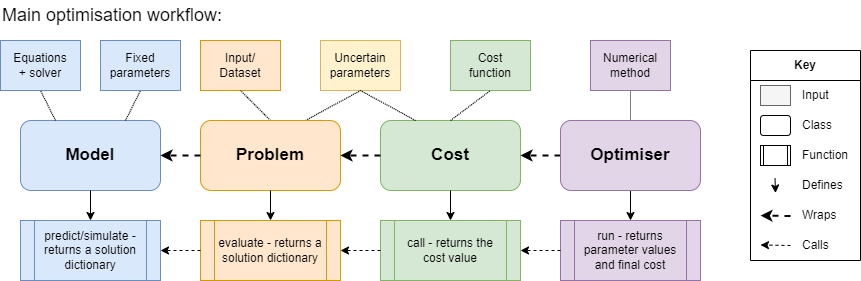
\includegraphics[width=0.8\textwidth,height=\textheight]{figures/PyBOP_components.drawio.png}
\caption{The core \texttt{PyBOP} architecture with base class
interfaces. Each class provides a direct mapping to a step in the
optimisation workflow. \label{fig:classes}}
\end{figure}

\texttt{PyBOP} formulates the inference process into four key classes:
model, problem, cost (or likelihood), and optimiser (or sampler), as
shown in \autoref{fig:classes}. Each of these objects represents a base
class with child classes constructing specialised functionality for
different workflows. The model class constructs a \texttt{PyBaMM}
forward model with a specified set of equations, initial conditions,
spatial discretisation, and numerical solver. By composing
\texttt{PyBaMM} directly into \texttt{PyBOP}, specialised models can be
constructed alongside the standard models that can also be modified for
different inference tasks. One such example is spatial
re-discretisation, which is required when one or more geometric
parameters are being optimised. In this situation, \texttt{PyBOP}
rebuilds the \texttt{PyBaMM} model only when necessary, reducing the
total number of rebuilds, providing improved performance. Alongside
construction of the forward model, \texttt{PyBOP}'s model class provides
methods for obtaining sensitivities from the prediction, enabling
gradient-based optimisation. A forward prediction, along with its
corresponding sensitivities, is provided to the problem class for
processing and exception control. A standardised data structure is then
provided to the cost classes, which then computes a distance, design, or
likelihood-based metric for optimisation. For point-based optimisation,
the optimisers minimise the cost function or the negative log-likelihood
if a likelihood class is provided. Bayesian inference is provided by
sampler classes, which accept the \texttt{LogPosterior} class and sample
from it using \texttt{PINTS}-based Monte Carlo algorithms at the time of
submission. In the typical workflow, the classes in
\autoref{fig:classes} are constructed in sequence, from left to right in
the figure.

In addition to the core architecture, \texttt{PyBOP} provides several
specialised inference and optimisation features. One example is
parameter inference from electrochemical impedance spectroscopy (EIS)
simulations, where PyBOP discretises and linearises the EIS forward
model into a sparse mass matrix form with accompanying
auto-differentiated Jacobian. This is then translated into the frequency
domain, giving a direct solution to compute the input-output impedance.
In this situation, the forward models are constructed within the spatial
re-discretisation workflow, allowing for geometric parameter inference
from EIS simulations and data.

A second specialised feature is that \texttt{PyBOP} builds on the
\texttt{JAX} (\citeproc{ref-jax:2018}{Bradbury et al., 2018}) numerical
solvers used by \texttt{PyBaMM} by providing \texttt{JAX}-based cost
functions for automatic forward model differentiation with respect to
the parameters. This functionality provides a performance improvement
and allows users to harness many other JAX-based inference packages to
optimise cost functions, such as \texttt{Numpyro}
(\citeproc{ref-numpyro:2019}{Phan et al., 2019}), \texttt{BlackJAX}
(\citeproc{ref-blackjax:2024}{Cabezas et al., 2024}), and \texttt{Optax}
(\citeproc{ref-optax:2020}{DeepMind et al., 2020}).

The currently implemented subclasses for the model, problem, and cost
classes are listed in \autoref{tab:subclasses}. The model and optimiser
classes can be selected in combination with any problem-cost pair.

\begin{longtable}[]{@{}
  >{\raggedright\arraybackslash}p{(\columnwidth - 4\tabcolsep) * \real{0.4458}}
  >{\raggedright\arraybackslash}p{(\columnwidth - 4\tabcolsep) * \real{0.2048}}
  >{\raggedright\arraybackslash}p{(\columnwidth - 4\tabcolsep) * \real{0.3494}}@{}}
\caption{List of available model, problem and cost (or likelihood)
classes. \label{tab:subclasses}}\tabularnewline
\toprule\noalign{}
\begin{minipage}[b]{\linewidth}\raggedright
Battery Models
\end{minipage} & \begin{minipage}[b]{\linewidth}\raggedright
Problem Types
\end{minipage} & \begin{minipage}[b]{\linewidth}\raggedright
Cost / Likelihood Functions
\end{minipage} \\
\midrule\noalign{}
\endfirsthead
\toprule\noalign{}
\begin{minipage}[b]{\linewidth}\raggedright
Battery Models
\end{minipage} & \begin{minipage}[b]{\linewidth}\raggedright
Problem Types
\end{minipage} & \begin{minipage}[b]{\linewidth}\raggedright
Cost / Likelihood Functions
\end{minipage} \\
\midrule\noalign{}
\endhead
\bottomrule\noalign{}
\endlastfoot
Single-particle model (SPM) & Fitting problem & Sum-squared error \\
SPM with electrolyte (SPMe) & Design problem & Root-mean-squared
error \\
Doyle-Fuller-Newman (DFN) & Observer & Minkowski \\
Many-particle model (MPM) & & Sum-of-power \\
Multi-species multi-reaction (MSMR) & & Gaussian log likelihood \\
Weppner Huggins & & Maximum a posteriori \\
Equivalent circuit model (ECM) & & Volumetric energy density \\
& & Gravimetric energy density \\
\end{longtable}

Similarly, the current algorithms available for optimisation are
presented in \autoref{tab:optimisers}. It should be noted that SciPy
minimize includes several gradient and non-gradient methods. From here
on, the point-based parameterisation and design-optimisation tasks will
simply be referred to as optimisation tasks. This simplification can be
justified by comparing \autoref{eqn:parameterisation} and
\autoref{eqn:design}; deterministic parameterisation is just an
optimisation task to minimise a distance-based cost between model output
and measured values.

\begin{longtable}[]{@{}
  >{\raggedright\arraybackslash}p{(\columnwidth - 4\tabcolsep) * \real{0.4359}}
  >{\raggedright\arraybackslash}p{(\columnwidth - 4\tabcolsep) * \real{0.3333}}
  >{\raggedright\arraybackslash}p{(\columnwidth - 4\tabcolsep) * \real{0.2308}}@{}}
\caption{Currently supported optimisers classified by candidate solution
type, including gradient information.
\label{tab:optimisers}}\tabularnewline
\toprule\noalign{}
\begin{minipage}[b]{\linewidth}\raggedright
Gradient-based
\end{minipage} & \begin{minipage}[b]{\linewidth}\raggedright
Evolutionary
\end{minipage} & \begin{minipage}[b]{\linewidth}\raggedright
(Meta)heuristic
\end{minipage} \\
\midrule\noalign{}
\endfirsthead
\toprule\noalign{}
\begin{minipage}[b]{\linewidth}\raggedright
Gradient-based
\end{minipage} & \begin{minipage}[b]{\linewidth}\raggedright
Evolutionary
\end{minipage} & \begin{minipage}[b]{\linewidth}\raggedright
(Meta)heuristic
\end{minipage} \\
\midrule\noalign{}
\endhead
\bottomrule\noalign{}
\endlastfoot
Weight decayed adaptive moment estimation (AdamW) & Covariance matrix
adaptation (CMA-ES) & Particle swarm (PSO) \\
Improved resilient backpropagation (iRProp-) & Exponential natural
(xNES) & Nelder-Mead \\
Gradient descent & Separable natural (sNES) & Cuckoo search \\
SciPy minimize & SciPy differential evolution & \\
\end{longtable}

In addition to deterministic optimisers \autoref{tab:subclasses},
\texttt{PyBOP} also provides Monte Carlo sampling routines to estimate
distributions of parameters within a Bayesian framework. These methods
construct a posterior parameter distribution that can be used to assess
uncertainty and practical identifiability. The individual sampler
classes are currently composed within \texttt{PyBOP} from the
\texttt{PINTS} library, with a base sampler class implemented for
interoperability and direct integration with \texttt{PyBOP}'s model,
problem, and likelihood classes. The currently supported samplers are
listed in \autoref{tab:samplers}.

\begin{longtable}[]{@{}
  >{\raggedright\arraybackslash}p{(\columnwidth - 8\tabcolsep) * \real{0.1624}}
  >{\raggedright\arraybackslash}p{(\columnwidth - 8\tabcolsep) * \real{0.2393}}
  >{\raggedright\arraybackslash}p{(\columnwidth - 8\tabcolsep) * \real{0.1368}}
  >{\raggedright\arraybackslash}p{(\columnwidth - 8\tabcolsep) * \real{0.2051}}
  >{\raggedright\arraybackslash}p{(\columnwidth - 8\tabcolsep) * \real{0.2564}}@{}}
\caption{Sampling methods supported by \texttt{PyBOP}, classified
according to the proposed method. \label{tab:samplers}}\tabularnewline
\toprule\noalign{}
\begin{minipage}[b]{\linewidth}\raggedright
Gradient-based
\end{minipage} & \begin{minipage}[b]{\linewidth}\raggedright
Adaptive
\end{minipage} & \begin{minipage}[b]{\linewidth}\raggedright
Slicing
\end{minipage} & \begin{minipage}[b]{\linewidth}\raggedright
Evolutionary
\end{minipage} & \begin{minipage}[b]{\linewidth}\raggedright
Other
\end{minipage} \\
\midrule\noalign{}
\endfirsthead
\toprule\noalign{}
\begin{minipage}[b]{\linewidth}\raggedright
Gradient-based
\end{minipage} & \begin{minipage}[b]{\linewidth}\raggedright
Adaptive
\end{minipage} & \begin{minipage}[b]{\linewidth}\raggedright
Slicing
\end{minipage} & \begin{minipage}[b]{\linewidth}\raggedright
Evolutionary
\end{minipage} & \begin{minipage}[b]{\linewidth}\raggedright
Other
\end{minipage} \\
\midrule\noalign{}
\endhead
\bottomrule\noalign{}
\endlastfoot
Monomial gamma & Delayed rejection adaptive & Rank shrinking &
Differential evolution & Metropolis random walk \\
No-U-turn & Haario Bardenet & Doubling & & Emcee hammer \\
Hamiltonian & Haario & Stepout & & Metropolis adjusted Langevin \\
Relativistic & Rao Blackwell & & & \\
\end{longtable}

\section{Background}\label{background}

\subsection{Battery models}\label{battery-models}

In general, battery models (after spatial discretisation) can be written
in the form of a differential-algebraic system of equations,
\begin{equation}
\frac{\mathrm{d} \mathbf{x}}{\mathrm{d} t} = f(t,\mathbf{x},\mathbf{\theta}),
\label{dynamics}
\end{equation} \begin{equation}
0 = g(t, \mathbf{x}, \mathbf{\theta}),
\label{algebraic}
\end{equation} \begin{equation}
\mathbf{y}(t) = h(t, \mathbf{x}, \mathbf{\theta}),
\label{output}
\end{equation} with initial conditions \begin{equation}
\mathbf{x}(0) = \mathbf{x}_0(\mathbf{\theta}).
\label{initial_conditions}
\end{equation}

Here, \(t\) is time, \(\mathbf{x}(t)\) are the (spatially discretised)
states, \(\mathbf{y}(t)\) are the outputs (e.g.~the terminal voltage)
and \(\mathbf{\theta}\) are the unknown parameters.

Common battery models include various types of equivalent circuit models
(e.g.~the Thévenin model), the Doyle--Fuller--Newman (DFN) model
(\citeproc{ref-Doyle:1993}{Doyle et al., 1993};
\citeproc{ref-Fuller:1994}{Fuller et al., 1994}) based on porous
electrode theory, and its reduced-order variants including the single
particle model (SPM) (\citeproc{ref-Planella:2022}{Brosa Planella et
al., 2022}) and the multi-species multi-reaction (MSMR) model
(\citeproc{ref-Verbrugge:2017}{Verbrugge et al., 2017}). Simplified
models that retain acceptable predictive accuracy at lower computational
cost are widely used, for example in battery management systems, while
physics-based models are required to understand the impact of physical
parameters on performance. This separation of complexity traditionally
results in multiple parameterisations for a single battery type,
depending on the model structure.

\section{Examples}\label{examples}

\subsection{Parameterisation}\label{parameterisation}

The parameterisation of battery models is challenging due to the large
number of parameters that need to be identified compared to the number
of measurable outputs (\citeproc{ref-Andersson:2022}{Andersson et al.,
2022}; \citeproc{ref-Miguel:2021}{Miguel et al., 2021};
\citeproc{ref-Wang:2022}{Wang et al., 2022}). A complete
parameterisation often requires stepwise identification of smaller sets
of parameters from a variety of excitations and different data sets
(\citeproc{ref-Chen:2020}{Chen et al., 2020};
\citeproc{ref-Chu:2019}{Chu et al., 2019}; \citeproc{ref-Kirk:2022}{Kirk
et al., 2023}; \citeproc{ref-Lu:2021}{Lu et al., 2021}). Furthermore,
parameter identifiability can be poor for a given set of excitations and
data sets, requiring improved experimental design in addition to
uncertainty capable identification methods
(\citeproc{ref-Aitio:2020}{Aitio et al., 2020}).

A generic data-fitting optimisation problem may be formulated as:
\begin{equation}
\min_{\mathbf{\theta}} ~ \mathcal{L}_{(\hat{\mathbf{y}_i})}(\mathbf{\theta}) ~~~
\textrm{subject to equations (\ref{dynamics})\textrm{-}(\ref{initial_conditions})}
\label{eqn:parameterisation}
\end{equation}

where \(\mathcal{L} : \mathbf{\theta} \mapsto [0,\infty)\) is a cost
function that quantifies the agreement between the model output
\(\mathbf{y}(t)\) and a sequence of observations
\((\hat{\mathbf{y}_i})\) measured at times \(t_i\). Within the
\texttt{PyBOP} framework, the \texttt{FittingProblem} class packages the
model output along with the measured observations, both of which are
then passed to the cost classes for the computation of the specific cost
function. For gradient-based optimisers, the Jacobian of the cost
function with respect to unknown parameters,
\(\partial \mathcal{L} / \partial \theta\), is computed for step-size
and directional information.

Next, we demonstrate the fitting of synthetic data where the model
parameters are known. Throughout this section, as an example, we use
\texttt{PyBaMM}'s implementation of the single particle model with an
added contact resistance submodel. We assume that the model is already
fully parameterised apart from two dynamic parameters, namely, the
lithium diffusivity of the negative electrode active material particles
(denoted ``negative particle diffusivity'') and the contact resistance
with corresponding true values of {[}3.3e-14 \(\text{m}^2/\text{s}\), 10
mOhm{]}. We generate synthetic data with a one-hour discharge from 100\%
to 0\% state of charge, denoted as 1C rate, followed by 30 minutes of
relaxation. This dataset is then corrupted with zero-mean Gaussian noise
of amplitude 2 mV, with the resulting signal shown by the blue dots in
\autoref{fig:inference-time-landscape} (left). The initial states are
assumed known, although this assumption is not generally necessary. The
\texttt{PyBOP} repository contains several other
\href{https://github.com/pybop-team/PyBOP/tree/develop/examples/notebooks}{example
notebooks} that follow a similar inference process. The underlying cost
landscape to be explored by the optimiser is shown in
\autoref{fig:inference-time-landscape} (right), with the initial
position denoted alongside the known true system parameters for this
synthetic inference task. In general, the true parameters are not known.

\begin{figure}
\centering
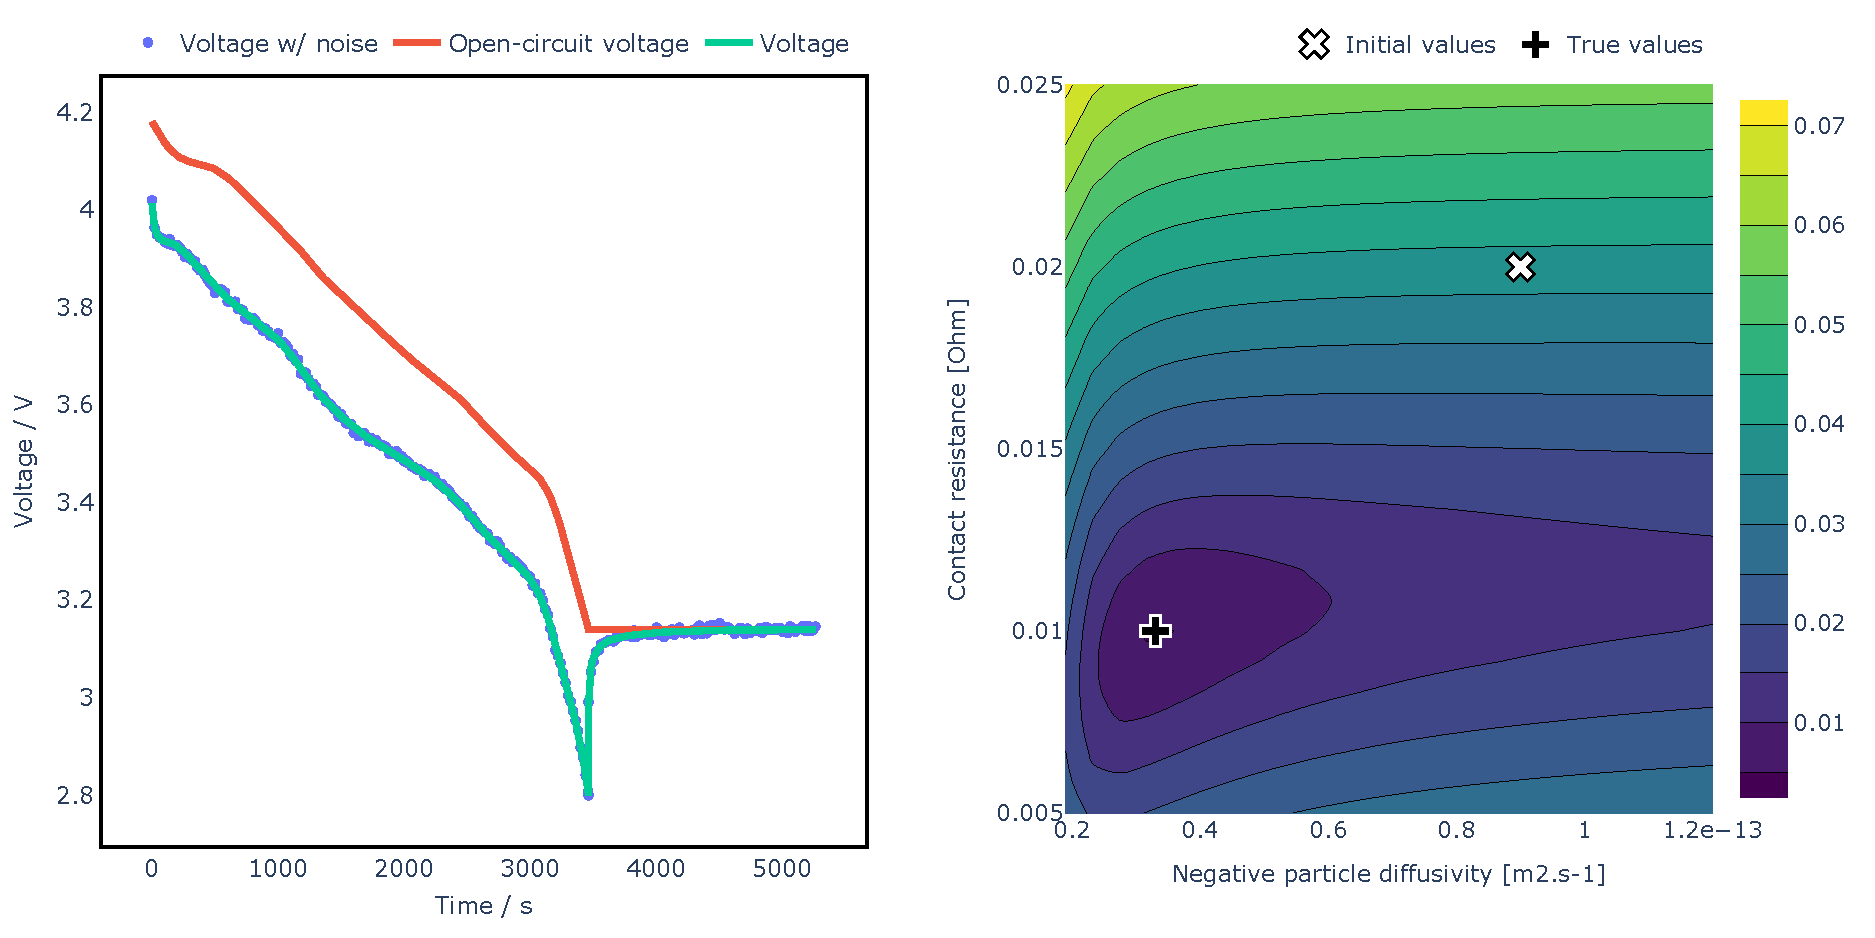
\includegraphics[width=1\textwidth,height=\textheight]{figures/joss/sim-landscape.pdf}
\caption{The synthetic fitting dataset (left) and cost landscape (right)
for an example time-series battery model parameterisation using a
root-mean-squared error cost function.
\label{fig:inference-time-landscape}}
\end{figure}

Using the same model and parameters, we now showcase \texttt{PyBOP}'s
capability to fit electrochemical impedance data using methods within
\texttt{pybamm-eis} that enable fast impedance computation of battery
models (\citeproc{ref-pybamm-eis}{Dhoot et al., 2024}).
\autoref{fig:impedance-landscape} shows the numerical impedance
prediction available in \texttt{PyBOP} alongside the cost landscape
constructed for the inference task. At the time of publication,
gradient-based optimisation and sampling methods are not available when
using an impedance workflow.

\begin{figure}
\centering
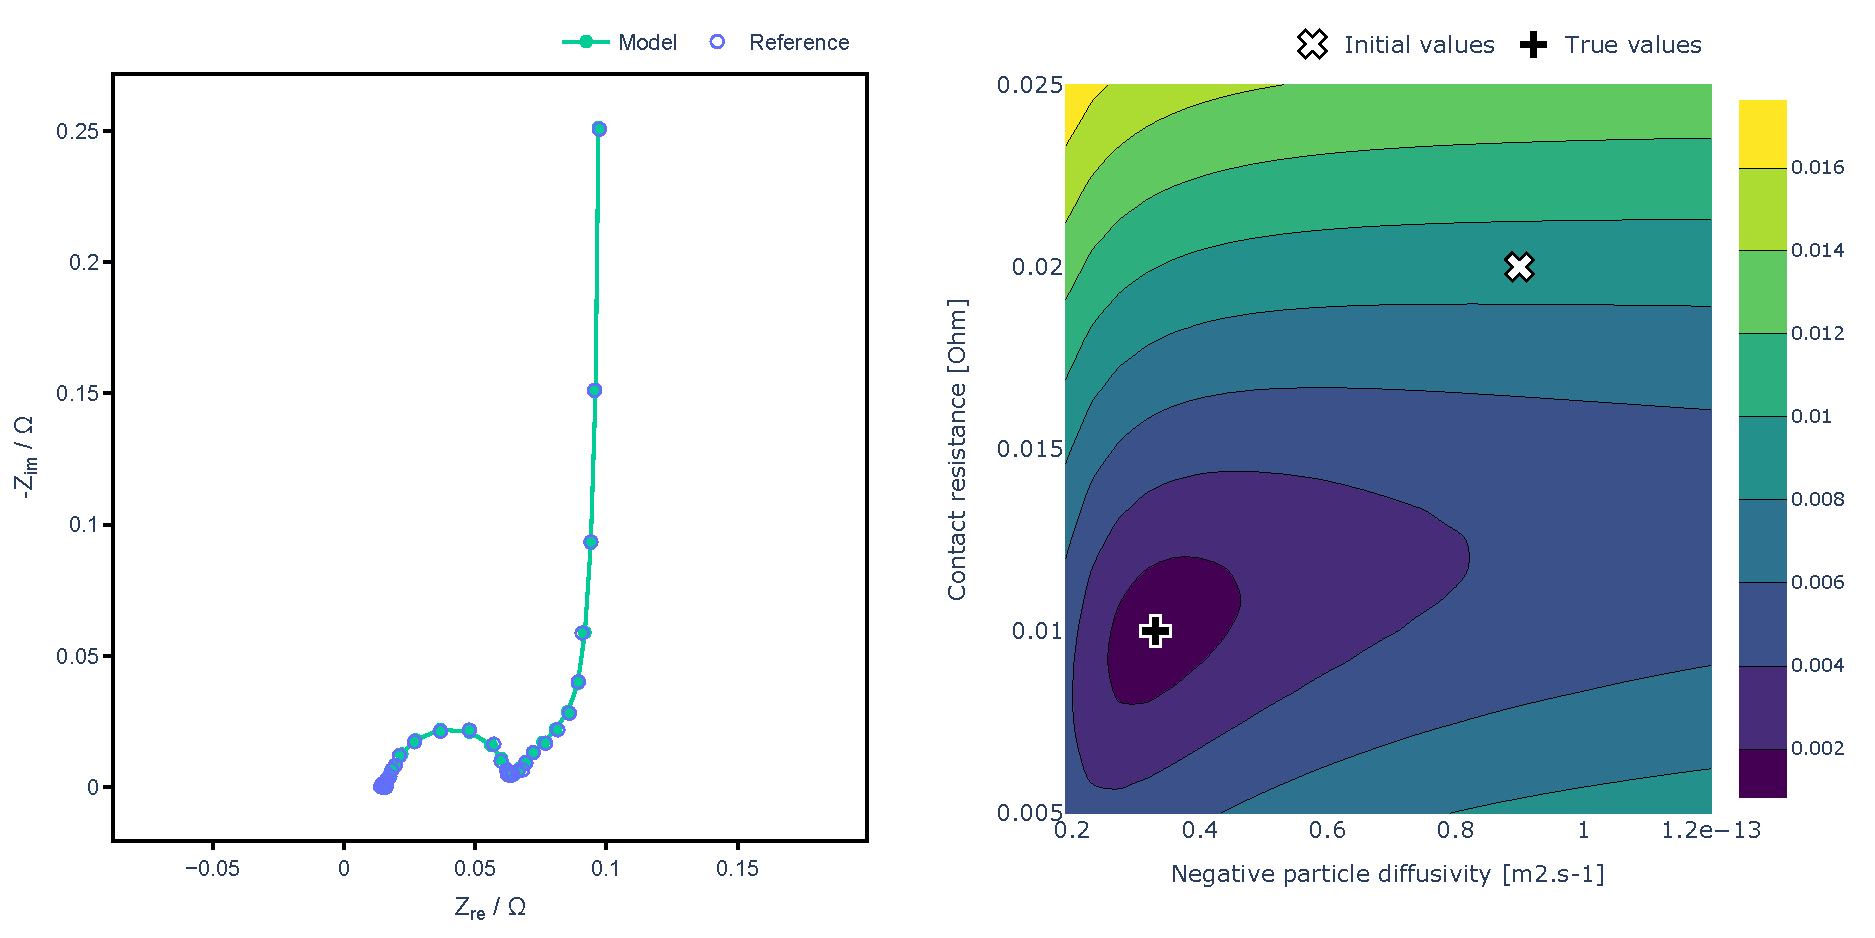
\includegraphics[width=1\textwidth,height=\textheight]{figures/joss/impedance.pdf}
\caption{The data and model fit (left) and cost landscape (right) for a
frequency-domain impedance parameterisation with a root-mean-squared
error cost function, at 5\% SOC. \label{fig:impedance-landscape}}
\end{figure}

To avoid confusion in the remainder of this section, we will continue
with identification of the example model in the time-domain. In general,
however, time- and frequency-domain models and data may be combined for
improved parameterisation. As gradient information is available for our
time-domain example, the choice of distance-based cost function and
optimiser is not constrained. Due to the difference in magnitude between
the two parameters, we apply the logarithmic parameter transformation
offered by \texttt{PyBOP}. This transforms the search space of the
optimiser to allow for a common step size between the parameters,
improving convergence in this particular case. As a demonstration of the
parameterisation capabilities of \texttt{PyBOP},
\autoref{fig:convergence-min-max} (left) shows the rate of convergence
for each of the distance-minimising cost functions, while
\autoref{fig:convergence-min-max} (right) shows analogous results for
maximising a likelihood. The optimisation is performed with SciPy
Minimize using the gradient-based L-BFGS-B method.

\begin{figure}
\centering
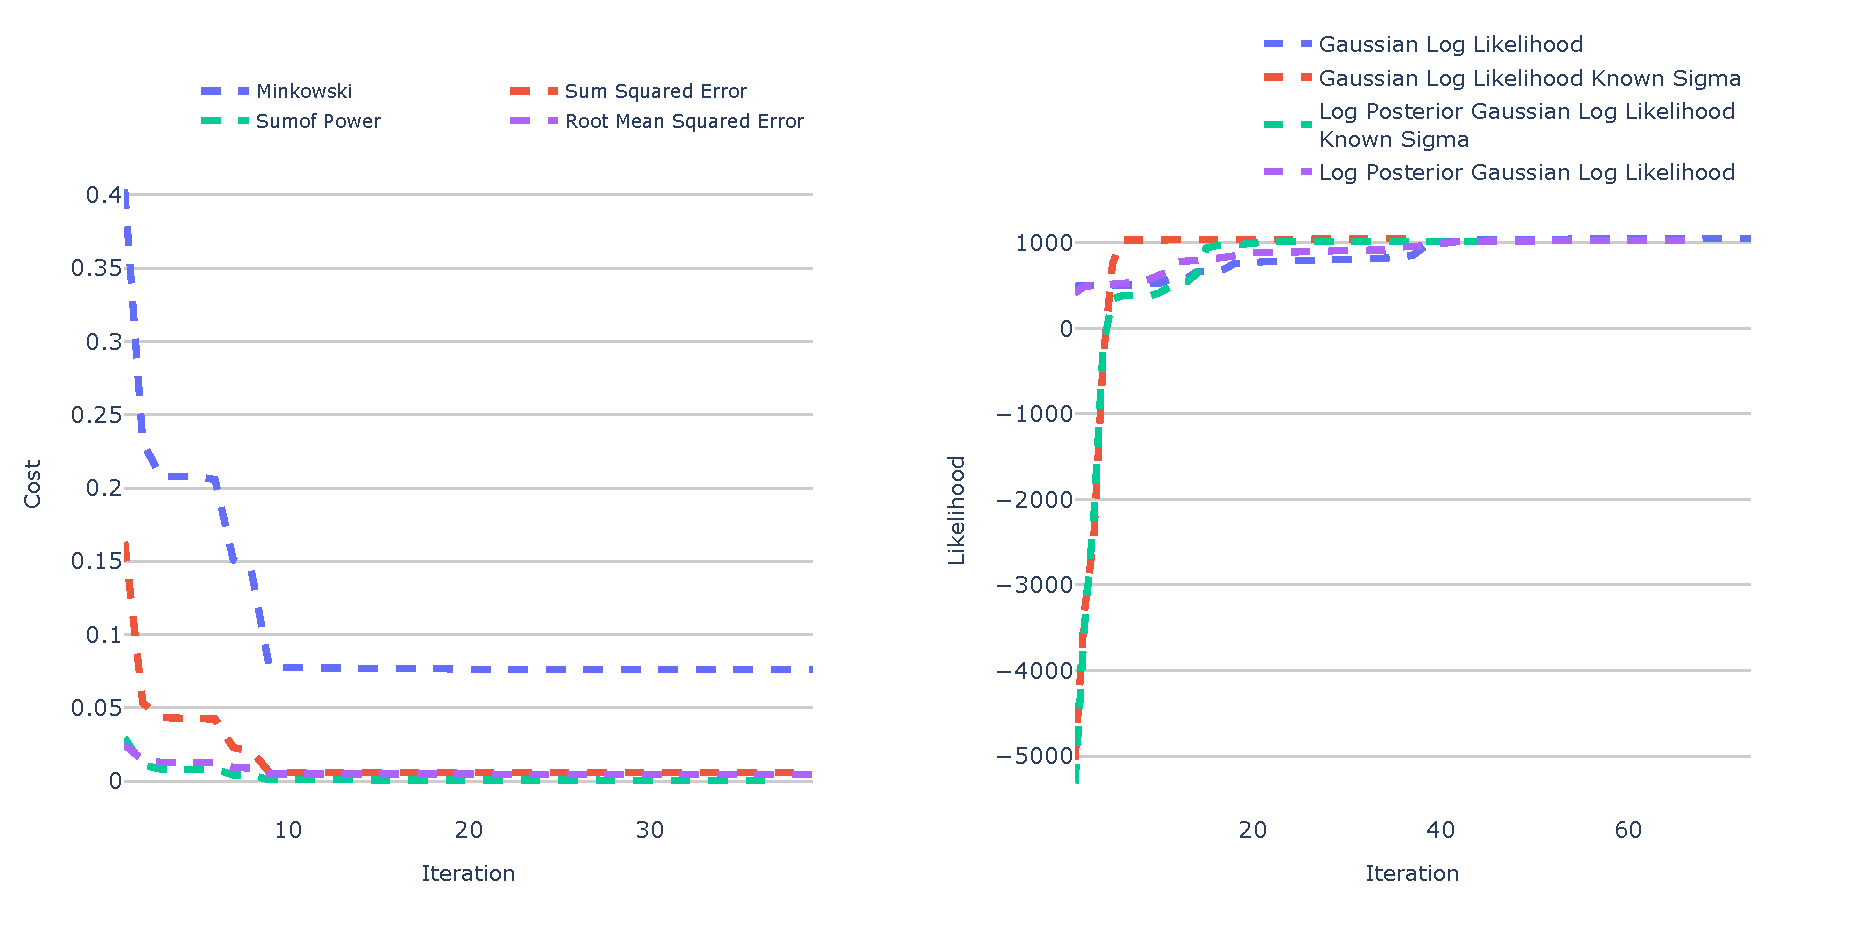
\includegraphics[width=1\textwidth,height=\textheight]{figures/joss/converge.pdf}
\caption{Optimiser convergence using various cost (left) and likelihood
(right) functions and the L-BFGS-B algorithm.
\label{fig:convergence-min-max}}
\end{figure}

We now show example optimiser convergence of various algorithms against
the same model and two parameters, across several categories:
gradient-based methods in \autoref{fig:optimiser-inference1} (left),
evolutionary strategies in \autoref{fig:optimiser-inference1} (middle)
and (meta)heuristics in \autoref{fig:optimiser-inference1} (right) using
a mean-squared-error cost function. We also show cost functions and
solution iterations in \autoref{fig:optimiser-inference2}, with the
three rows showing the gradient-based optimisers (top), evolution
strategies (middle), and (meta)heuristics (bottom). Note that the
performance of the optimiser depends on the cost environment, initial
guess or prior, and corresponding hyperparameters for each specific
problem.

\begin{figure}[htb]
\centering
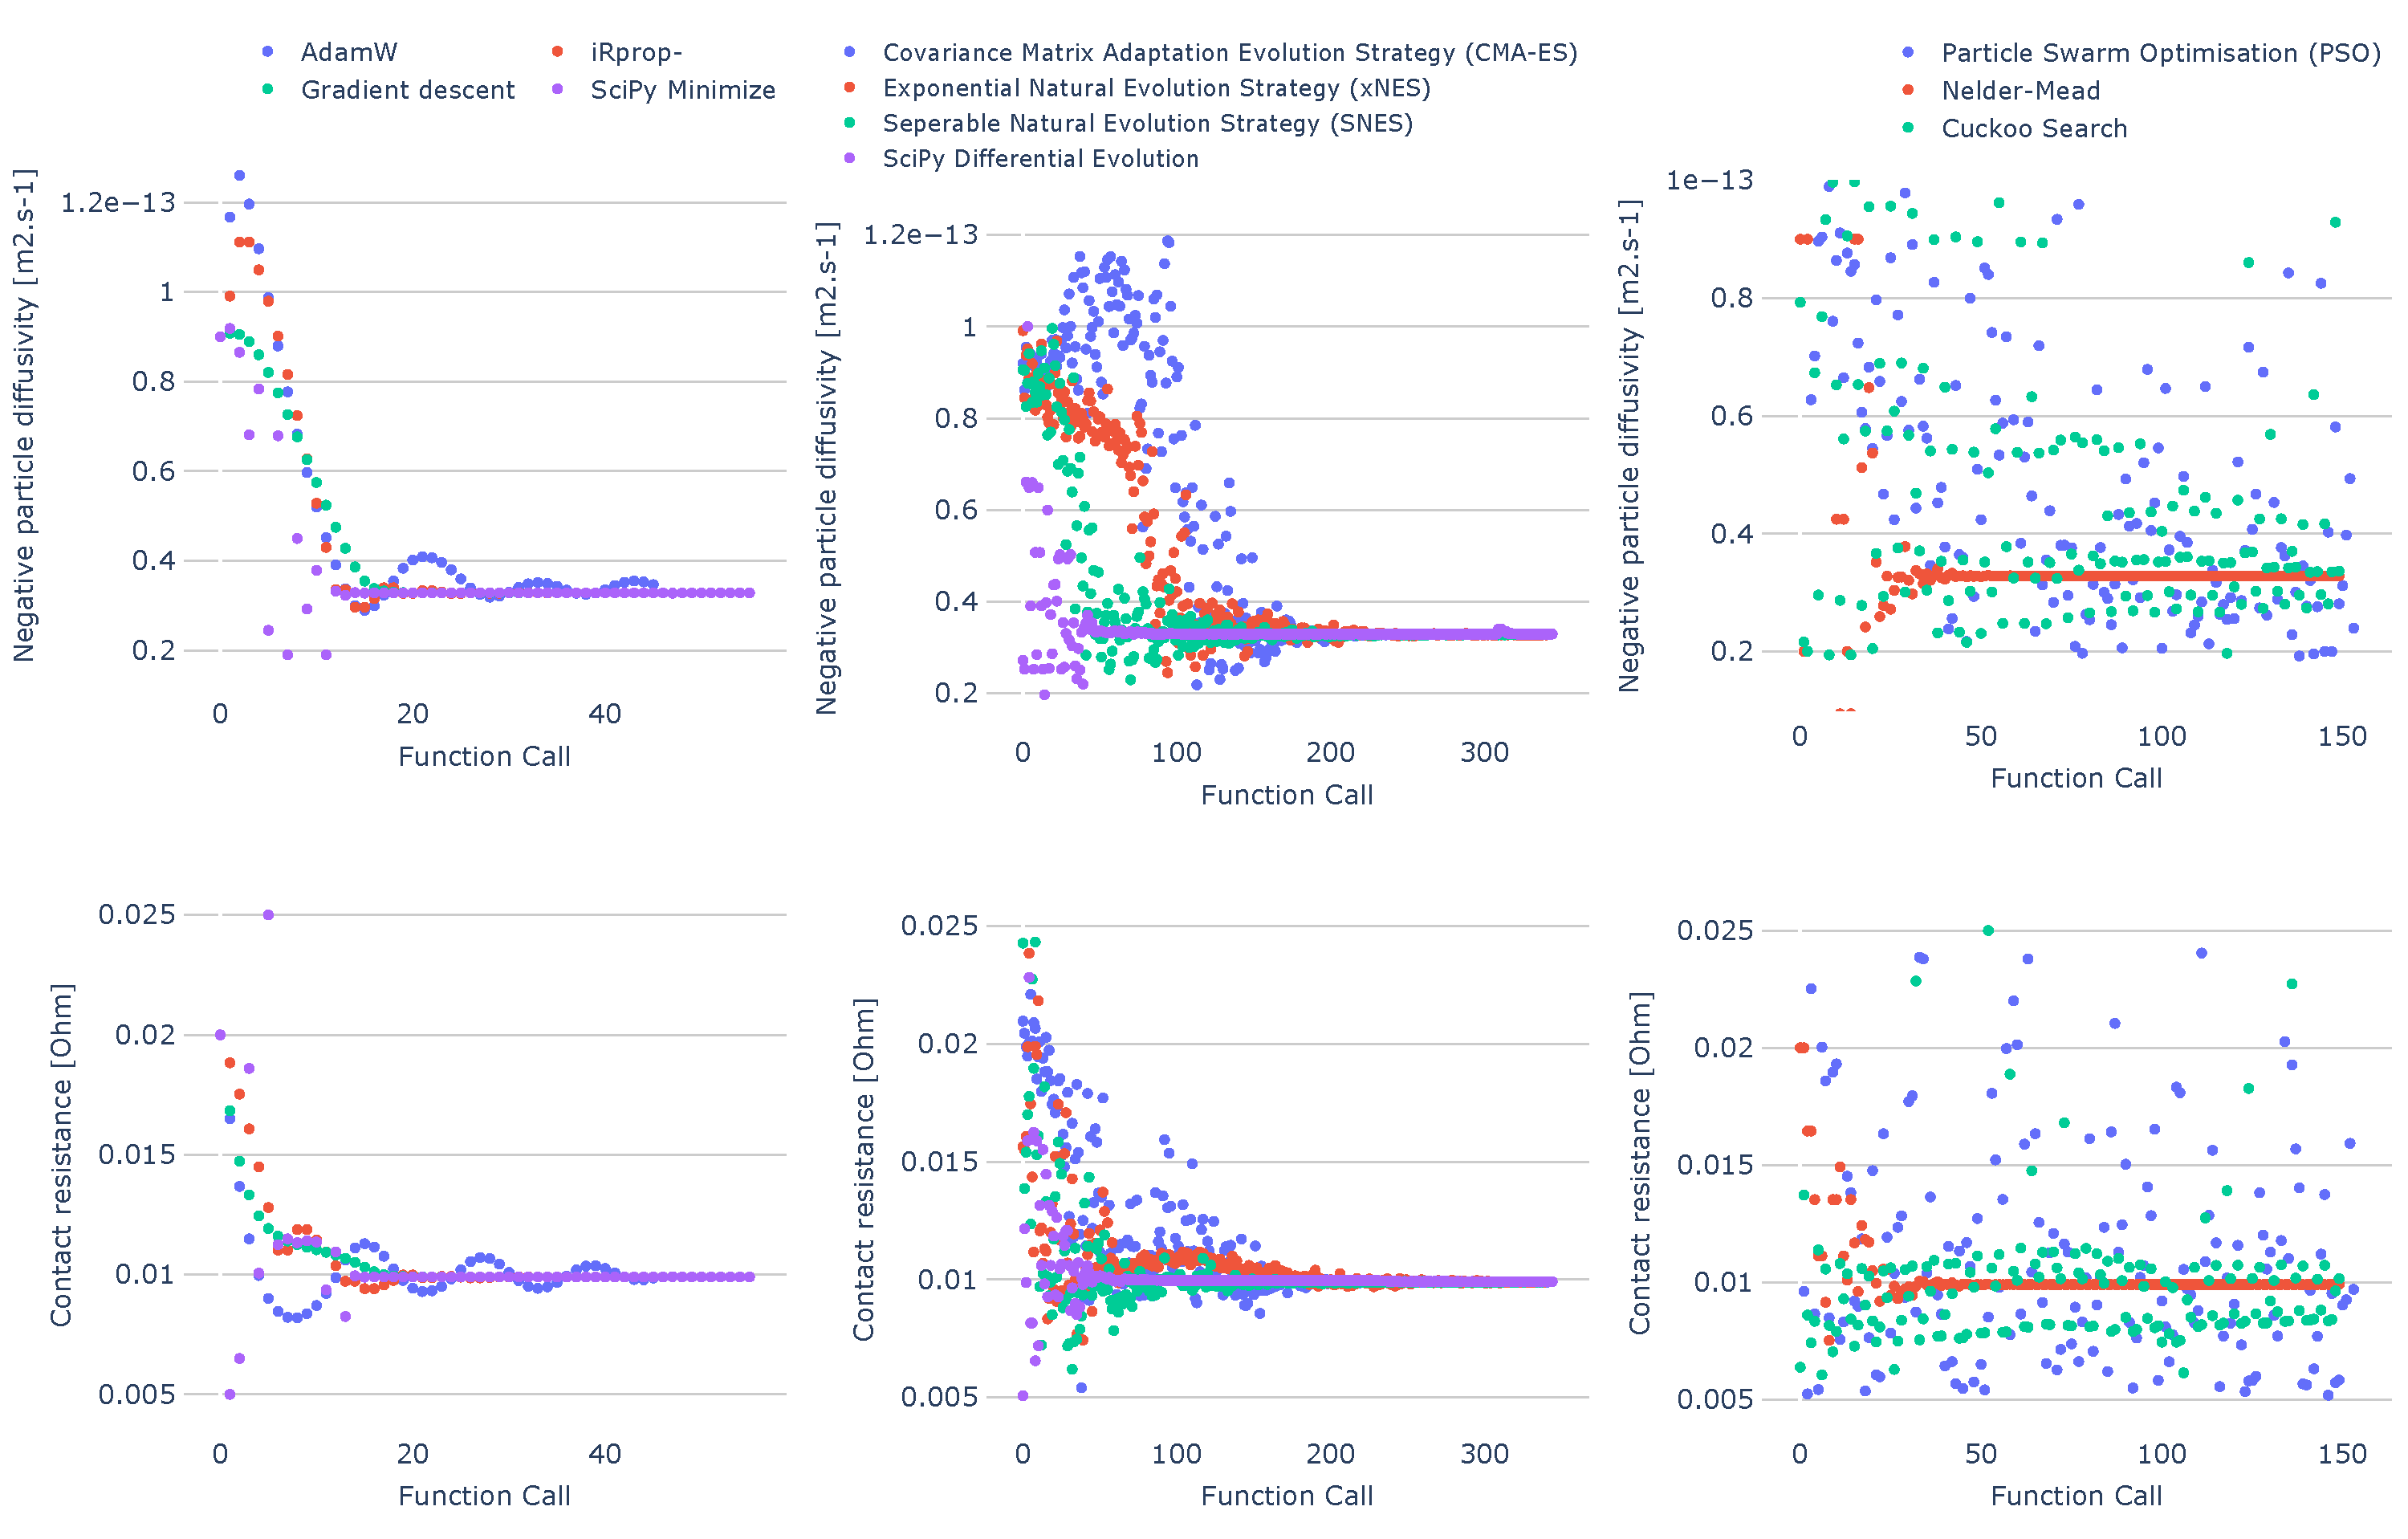
\includegraphics[width=1\textwidth,height=\textheight]{figures/joss/optimisers_parameters.pdf}
\caption{Convergence in parameter values for several optimisation
algorithms provided by \texttt{PyBOP}. \label{fig:optimiser-inference1}}
\end{figure}

\begin{figure}[htb]
\centering
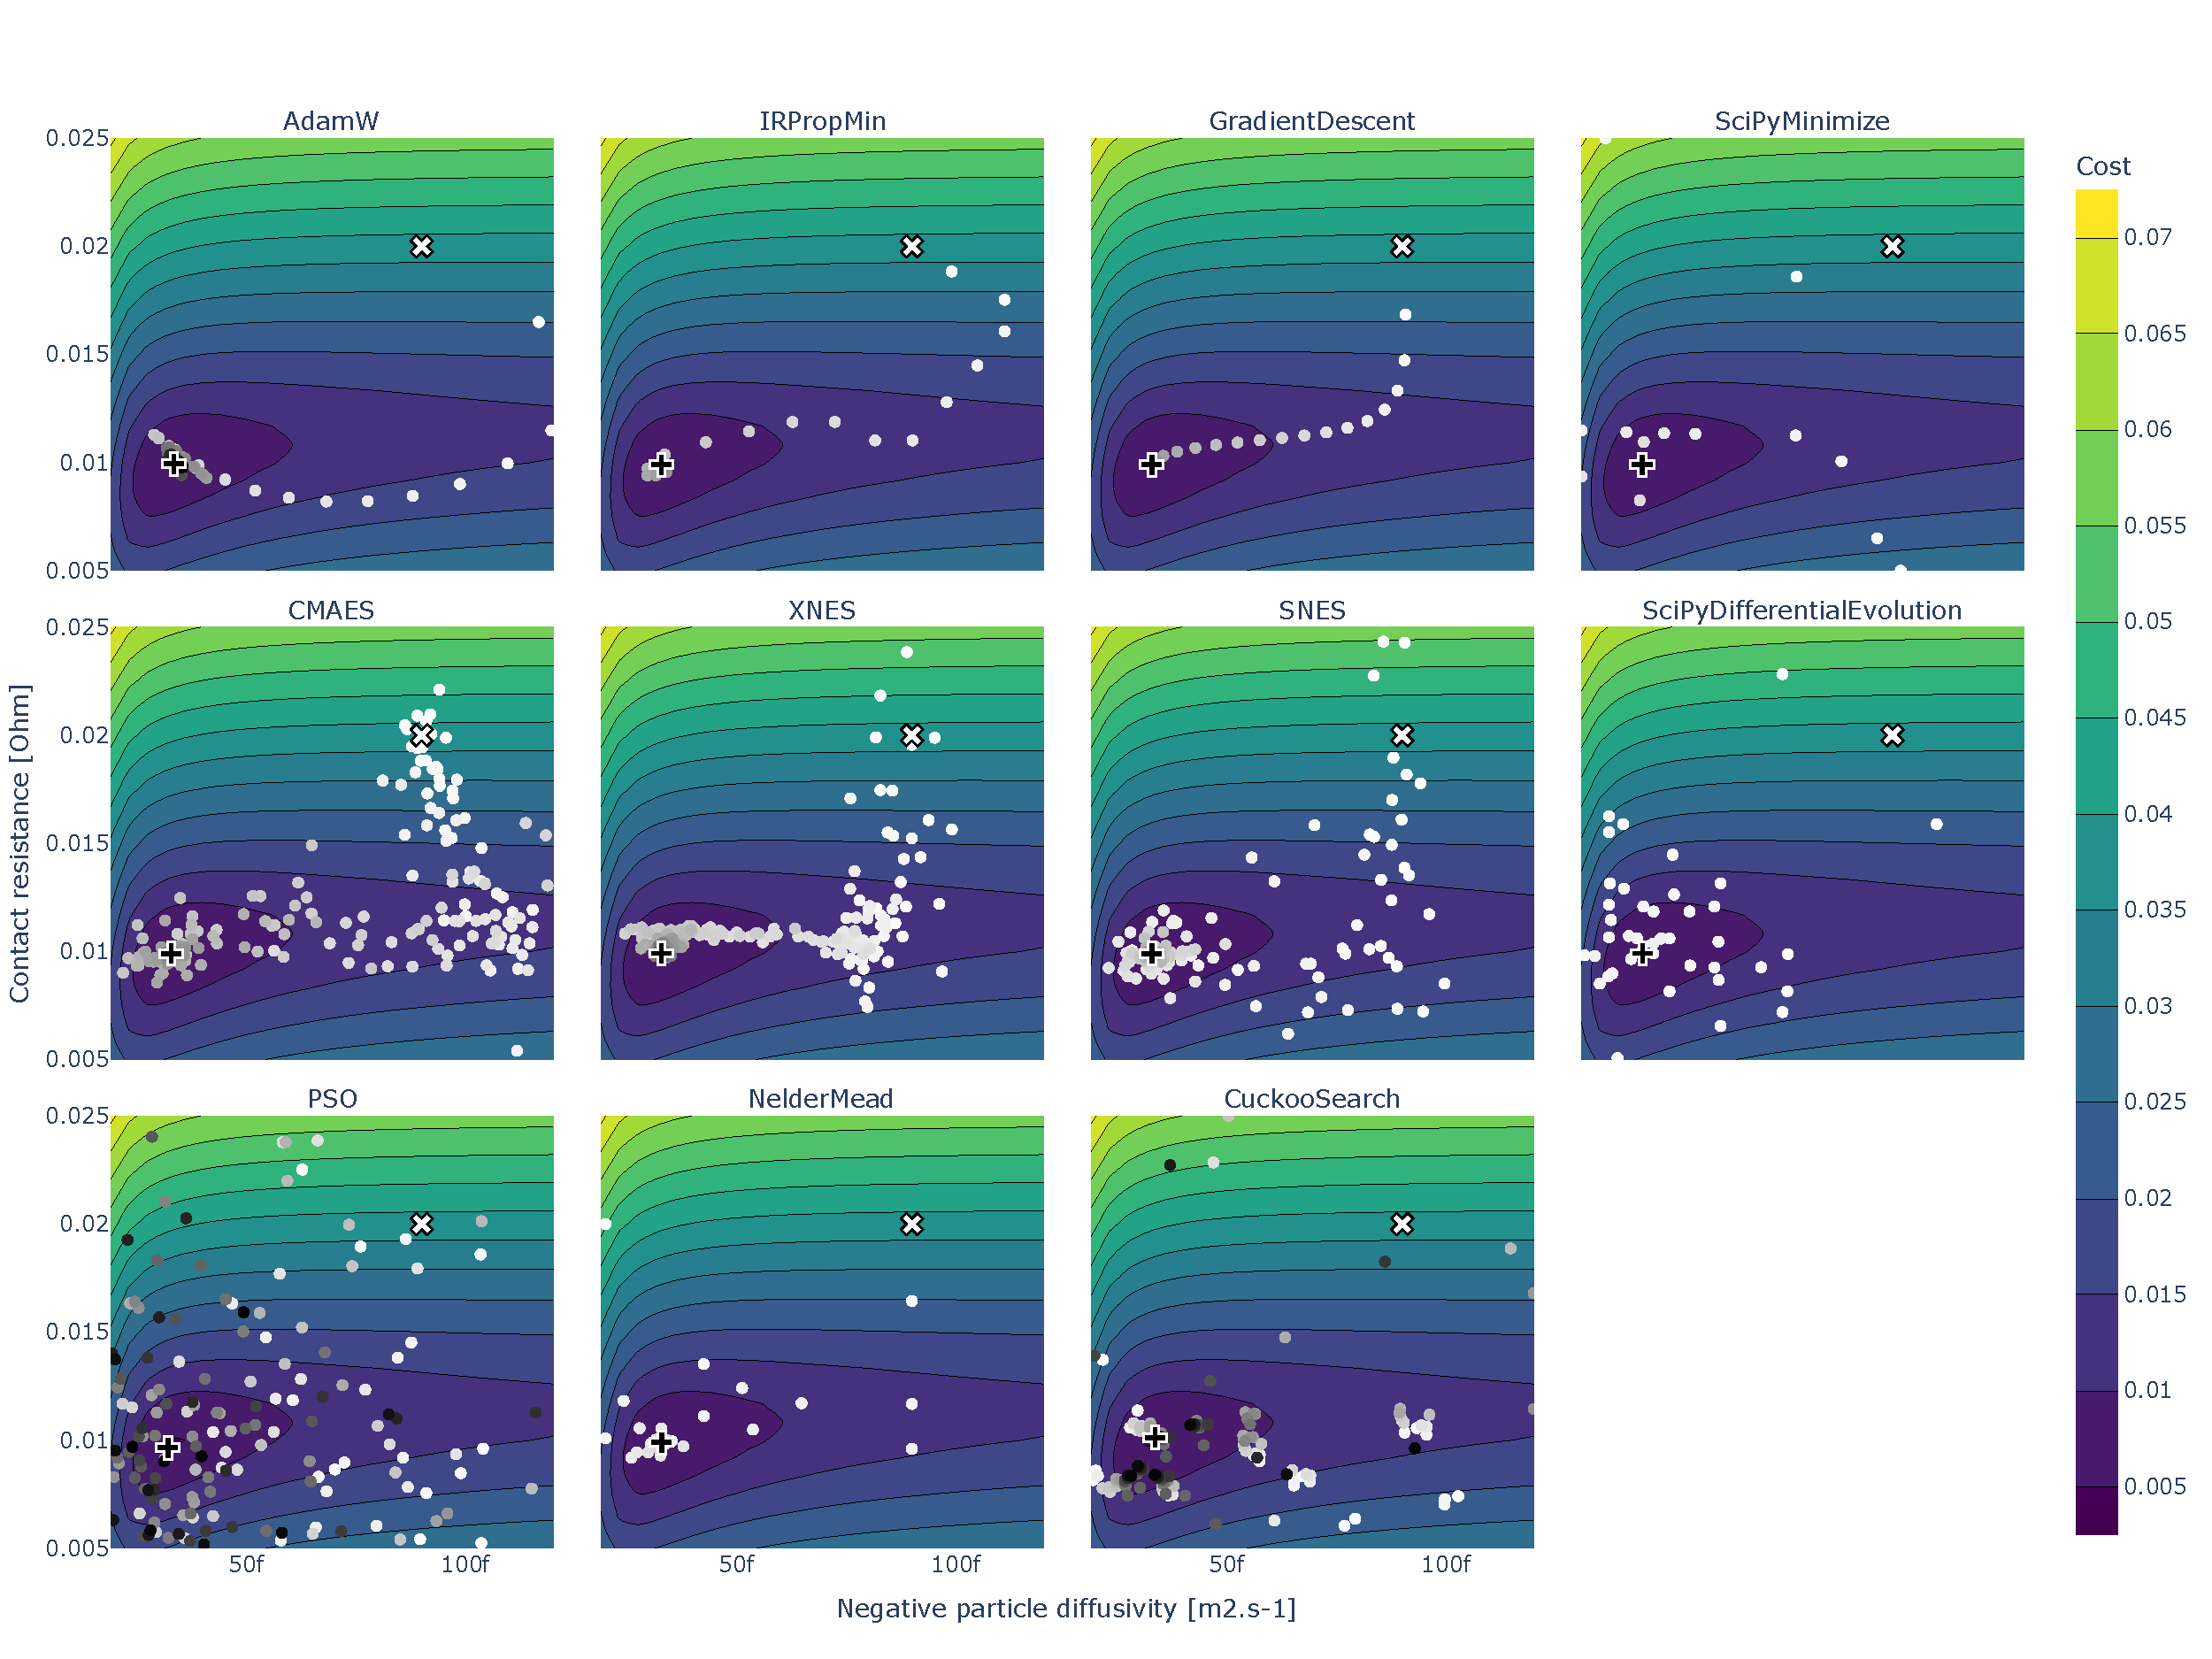
\includegraphics[width=1\textwidth,height=\textheight]{figures/joss/contour_subplot.pdf}
\caption{Cost landscape contour plot with corresponding optimisation
traces, for several optimisers. \label{fig:optimiser-inference2}}
\end{figure}

This example parameterisation task can also be approached from a
Bayesian perspective, solved using \texttt{PyBOP}`s sampler methods.
First, we introduce Bayes' rule,

\begin{equation}
P(\theta|D) = \frac{P(D|\theta)P(\theta)}{P(D)},
\label{eqn:bayes_theorem}
\end{equation}

where \(P(\theta|D)\) is the posterior parameter distribution,
\(P(D|\theta)\) is the likelihood function, \(P(\theta)\) is the prior
parameter distribution, and \(P(D)\) is the model evidence, or marginal
likelihood, which acts as a normalising constant. In the case of maximum
likelihood estimation or maximum a posteriori estimation, one wishes to
maximise \(P(D|\theta)\) or \(P(\theta|D)\), respectively, and this may
be formulated as an optimisation problem as per
\autoref{eqn:parameterisation}.

To estimate the full posterior parameter distribution, however, one must
use sampling or other inference methods to reconstruct the function
\(P(\theta|D)\). The posterior distribution provides information about
the uncertainty of the identified parameters, e.g., by calculating the
variance or other moments. Monte Carlo methods are used here to sample
from the posterior. The selection of Monte Carlo methods available in
\texttt{PyBOP} includes gradient-based methods such as no-u-turn
(\citeproc{ref-NUTS:2011}{Hoffman \& Gelman, 2011}) and Hamiltonian
(\citeproc{ref-Hamiltonian:2011}{Brooks et al., 2011}), as well as
heuristic methods such as differential evolution
(\citeproc{ref-DiffEvolution:2006}{Braak, 2006}), and also conventional
methods based on random sampling with rejection criteria
(\citeproc{ref-metropolis:1953}{Metropolis et al., 1953}).
\texttt{PyBOP} offers a sampler class that provides the interface to
samplers, the latter being provided by the probabilistic inference on
noisy time-series (\texttt{PINTS}) package. \autoref{fig:posteriors}
shows the sampled posteriors for the synthetic model described
previously, using an adaptive covariance-based sampler called Haario
Bardenet (\citeproc{ref-Haario:2001}{Haario et al., 2001}).

\begin{figure}
\centering
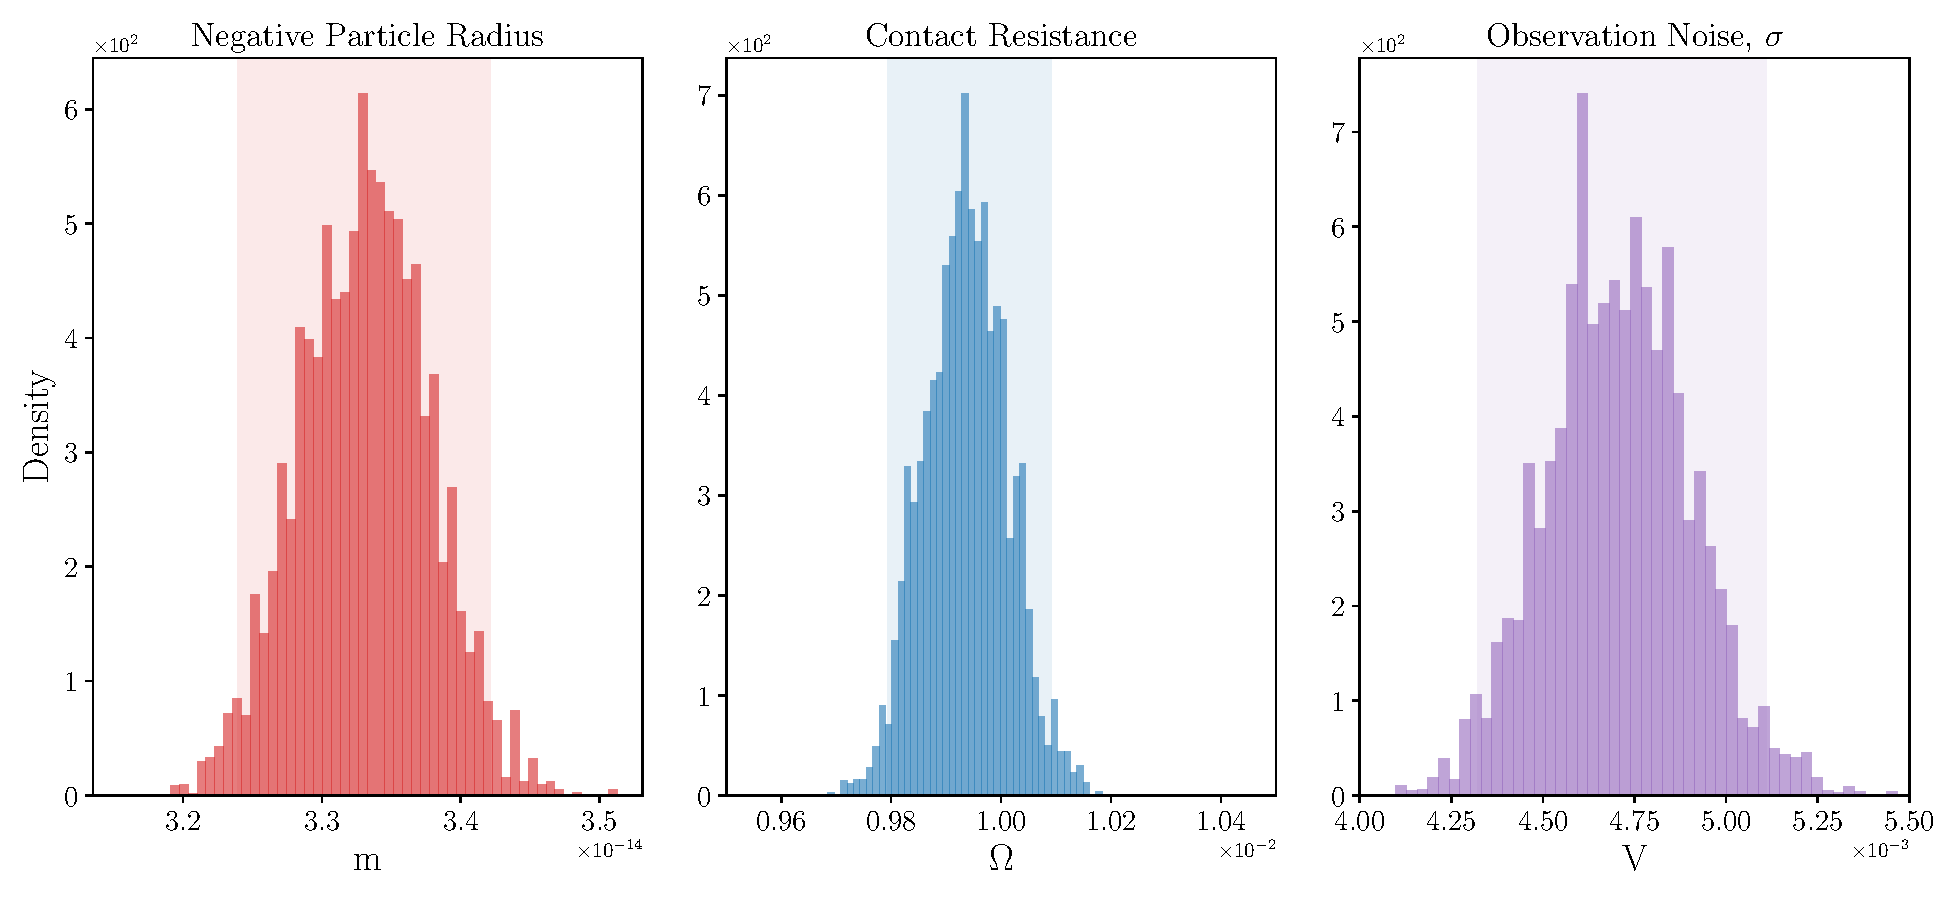
\includegraphics[width=1\textwidth,height=\textheight]{figures/joss/posteriors.pdf}
\caption{Posterior distributions of model parameters alongside
identified noise on the observations. Shaded area denotes the 95th
percentile credible interval for each parameter. \label{fig:posteriors}}
\end{figure}

\subsection{Design optimisation}\label{design-optimisation}

Design optimisation is supported in \texttt{PyBOP} to guide device
design development by identifying parameter sensitivities that can
unlock improvements in performance. This problem can be viewed in a
similar way to the parameterisation workflows described previously, but
with the aim of maximising a design-objective cost function rather than
minimising a distance cost function. \texttt{PyBOP} performs
maximisation by minimising the negative of the cost function. In design
problems, the cost metric is no longer a distance between two time
series, but a metric evaluated on a model prediction. For example, to
maximise the gravimetric energy (or power) density, the cost is the
integral of the discharge energy (or power) normalised by the cell mass.
Such metrics are typically quantified for operating conditions such as a
1C discharge, at a given temperature.

In general, design optimisation can be written as a constrained
optimisation problem, \begin{equation}
\min_{\mathbf{\theta} \in \Omega} ~ \mathcal{L}(\mathbf{\theta}) ~~~
\textrm{subject to equations (\ref{dynamics})\textrm{-}(\ref{initial_conditions}),}
\label{eqn:design}
\end{equation}

where \(\mathcal{L} : \mathbf{\theta} \mapsto [0,\infty)\) is a cost
function that quantifies the desirability of the design and \(\Omega\)
is the set of allowable parameter values.

As an example, we consider the challenge of maximising the gravimetric
energy density, subject to constraints on two of the geometric electrode
parameters (\citeproc{ref-Couto:2023}{Couto et al., 2023}). In this case
we use the \texttt{PyBaMM} implementation of the single particle model
with electrolyte (SPMe) to investigate the impact of the positive
electrode thickness and the active material volume fraction on the
energy density. Since the active material volume fraction and electrode
porosity sum to unity, the porosity for each optimisation iteration is
defined in relation to the volume fraction. In this problem, we estimate
the 1C rate from the theoretical capacity for each iteration of the
design and use the particle swarm optimisation algorithm.

\begin{figure}
\centering
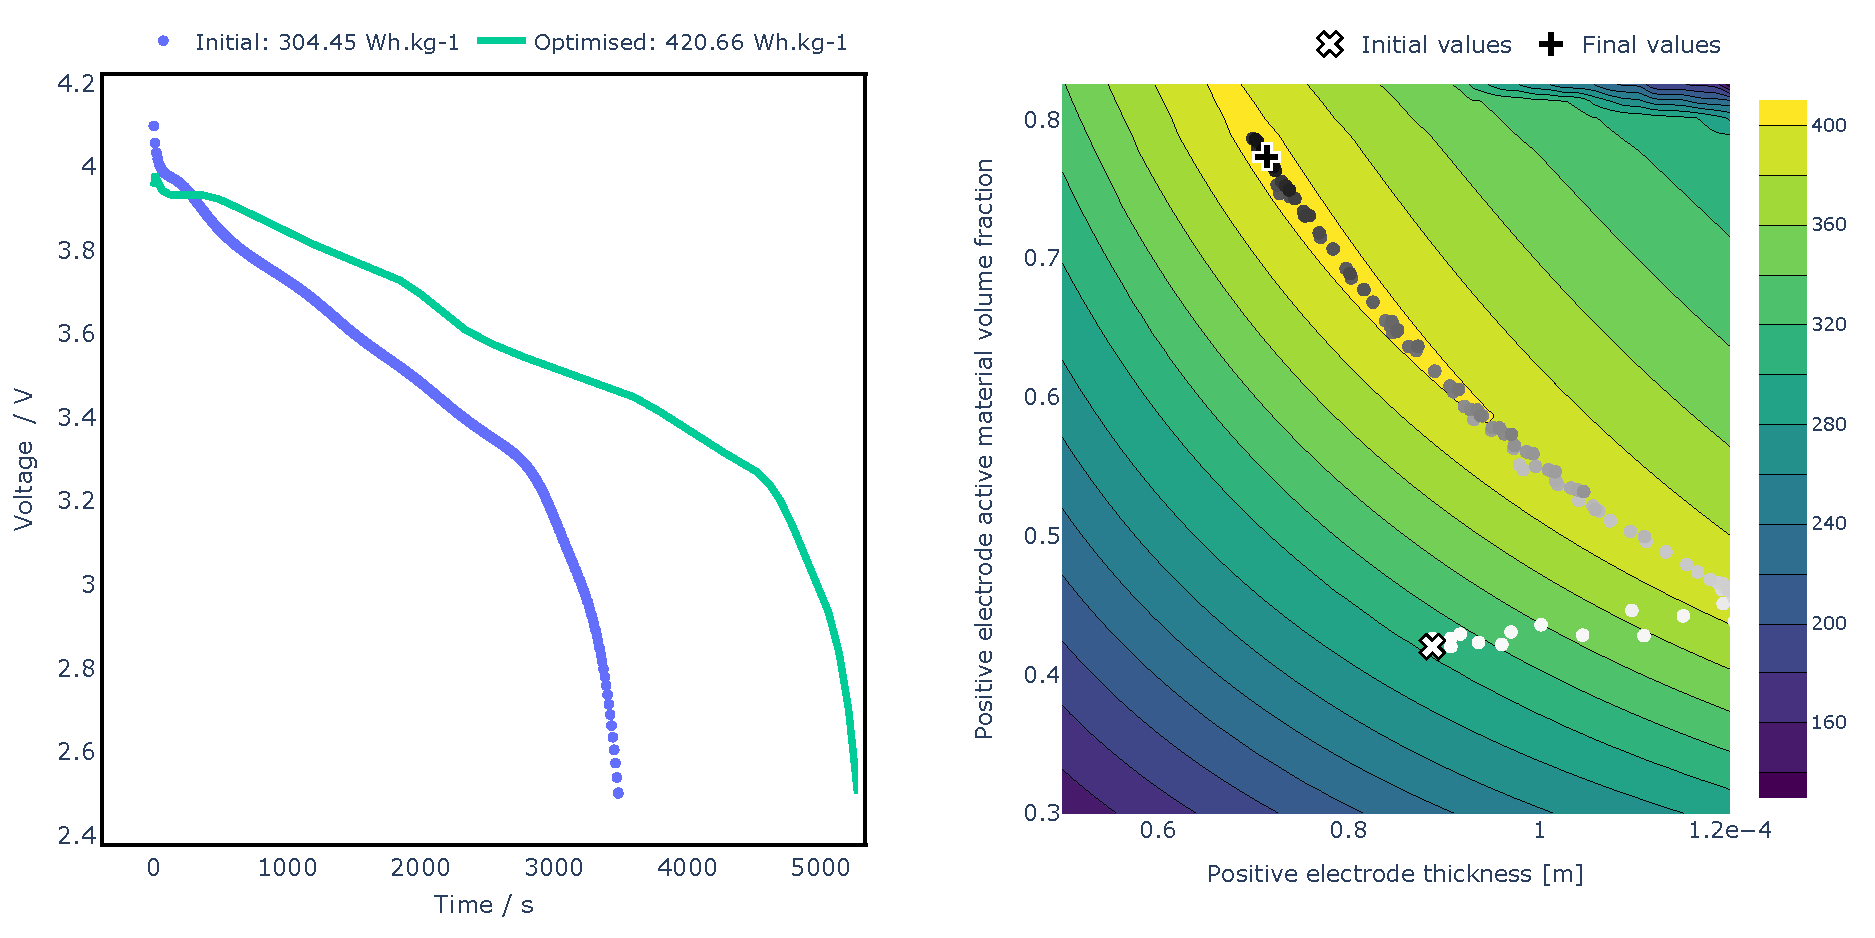
\includegraphics[width=1\textwidth,height=\textheight]{figures/joss/design.pdf}
\caption{Gravimetric energy density cost landscape alongside the initial
and optimised voltage profiles, for a fixed 1C discharge set from the
initial design. \label{fig:design_gravimetric}}
\end{figure}

\autoref{fig:design_gravimetric} (left) shows the Nelder-Mead search
over the parameter space and (right) the predicted improvement in the
discharge profile between the initial and optimised parameter values,
simulated at their respective 1C rates.

\section{Acknowledgements}\label{acknowledgements}

We gratefully acknowledge all
\href{https://github.com/pybop-team/PyBOP?tab=readme-ov-file\#contributors-}{contributors}
to \texttt{PyBOP}. This work was supported by the Faraday Institution
Multiscale Modelling project (ref. FIRG059), UKRI's Horizon Europe
Guarantee (ref. 10038031), and EU IntelLiGent project (ref. 101069765).

\section*{References}\label{references}
\addcontentsline{toc}{section}{References}

\phantomsection\label{refs}
\begin{CSLReferences}{1}{0}
\bibitem[\citeproctext]{ref-Aitio:2020}
Aitio, A., Marquis, S. G., Ascencio, P., \& Howey, D. (2020). Bayesian
parameter estimation applied to the li-ion battery single particle model
with electrolyte dynamicsa⁎this work was carried out with funding
received from the faraday institution (faraday.ac.uk; EP/S003053/1, ref.
FIRG003). Scott marquis was supported by the EPSRC centre for doctoral
training in industrially focused mathematical modelling (EP/L015803/1)
in collaboration with siemens corporate technology.
\emph{IFAC-PapersOnLine}, \emph{53}(2), 12497--12504.
https://doi.org/\url{https://doi.org/10.1016/j.ifacol.2020.12.1770}

\bibitem[\citeproctext]{ref-Andersson:2022}
Andersson, M., Streb, M., Ko, J. Y., Löfqvist Klass, V., Klett, M.,
Ekström, H., Johansson, M., \& Lindbergh, G. (2022). Parametrization of
physics-based battery models from input-output data: {A} review of
methodology and current research. \emph{Journal of Power Sources},
\emph{521}(November 2021), 230859.
\url{https://doi.org/10.1016/j.jpowsour.2021.230859}

\bibitem[\citeproctext]{ref-DiffEvolution:2006}
Braak, C. J. F. T. (2006). A {Markov} {Chain} {Monte} {Carlo} version of
the genetic algorithm {Differential} {Evolution}: Easy {Bayesian}
computing for real parameter spaces. \emph{Statistics and Computing},
\emph{16}(3), 239--249. \url{https://doi.org/10.1007/s11222-006-8769-1}

\bibitem[\citeproctext]{ref-jax:2018}
Bradbury, J., Frostig, R., Hawkins, P., Johnson, M. J., Leary, C.,
Maclaurin, D., Necula, G., Paszke, A., VanderPlas, J., Wanderman-Milne,
S., \& Zhang, Q. (2018). \emph{{JAX}: Composable transformations of
{P}ython+{N}um{P}y programs} (Version 0.3.13).
\url{http://github.com/jax-ml/jax}

\bibitem[\citeproctext]{ref-Hamiltonian:2011}
Brooks, S., Gelman, A., Jones, G., \& Meng, X.-L. (2011). \emph{Handbook
of markov chain monte carlo}. Chapman; Hall/CRC.
\url{https://doi.org/10.1201/b10905}

\bibitem[\citeproctext]{ref-Planella:2022}
Brosa Planella, F., Ai, W., Boyce, A. M., Ghosh, A., Korotkin, I., Sahu,
S., Sulzer, V., Timms, R., Tranter, T. G., Zyskin, M., Cooper, S. J.,
Edge, J. S., Foster, J. M., Marinescu, M., Wu, B., \& Richardson, G.
(2022). {A Continuum of Physics-Based Lithium-Ion Battery Models
Reviewed}. \emph{Progress in Energy}, \emph{4}(4), 042003.
\url{https://doi.org/10.1088/2516-1083/ac7d31}

\bibitem[\citeproctext]{ref-blackjax:2024}
Cabezas, A., Corenflos, A., Lao, J., \& Louf, R. (2024). \emph{BlackJAX:
Composable {B}ayesian inference in {JAX}}.
\url{https://arxiv.org/abs/2402.10797}

\bibitem[\citeproctext]{ref-Cauchy:1847}
Cauchy, A., \& others. (1847). M{é}thode g{é}n{é}rale pour la
r{é}solution des systemes d'{é}quations simultan{é}es. \emph{Comp. Rend.
Sci. Paris}, \emph{25}(1847), 536--538.

\bibitem[\citeproctext]{ref-Chen:2020}
Chen, C.-H., Brosa Planella, F., O'Regan, K., Gastol, D., Widanage, W.
D., \& Kendrick, E. (2020). Development of experimental techniques for
parameterization of multi-scale lithium-ion battery models.
\emph{Journal of The Electrochemical Society}, \emph{167}(8), 080534.
\url{https://doi.org/10.1149/1945-7111/ab9050}

\bibitem[\citeproctext]{ref-Chu:2019}
Chu, Z., Plett, G. L., Trimboli, M. S., \& Ouyang, M. (2019). A
control-oriented electrochemical model for lithium-ion battery, {P}art
{I}: {L}umped-parameter reduced-order model with constant phase element.
\emph{Journal of Energy Storage}, \emph{25}(August), 100828.
\url{https://doi.org/10.1016/j.est.2019.100828}

\bibitem[\citeproctext]{ref-Clerx:2019}
Clerx, M., Robinson, M., Lambert, B., Lei, C. L., Ghosh, S., Mirams, G.
R., \& Gavaghan, D. J. (2019). Probabilistic inference on noisy time
series ({PINTS}). \emph{Journal of Open Research Software}, \emph{7}(1),
23. \url{https://doi.org/10.5334/jors.252}

\bibitem[\citeproctext]{ref-Couto:2023}
Couto, L. D., Charkhgard, M., Karaman, B., Job, N., \& Kinnaert, M.
(2023). Lithium-ion battery design optimization based on a dimensionless
reduced-order electrochemical model. \emph{Energy}, \emph{263}(PE),
125966. \url{https://doi.org/10.1016/j.energy.2022.125966}

\bibitem[\citeproctext]{ref-optax:2020}
DeepMind, Babuschkin, I., Baumli, K., Bell, A., Bhupatiraju, S., Bruce,
J., Buchlovsky, P., Budden, D., Cai, T., Clark, A., Danihelka, I.,
Dedieu, A., Fantacci, C., Godwin, J., Jones, C., Hemsley, R., Hennigan,
T., Hessel, M., Hou, S., \ldots{} Viola, F. (2020). \emph{The
{D}eep{M}ind {JAX} {E}cosystem}. \url{http://github.com/google-deepmind}

\bibitem[\citeproctext]{ref-pybamm-eis}
Dhoot, R., Timms, R., \& Please, C. (2024). \emph{PyBaMM EIS: Efficient
linear algebra methods to determine li-ion battery behaviour} (Version
0.1.4). \url{https://www.github.com/pybamm-team/pybamm-eis}

\bibitem[\citeproctext]{ref-Doyle:1993}
Doyle, M., Fuller, T. F., \& Newman, J. (1993). {Modeling of
Galvanostatic Charge and Discharge of the Lithium/Polymer/Insertion
Cell}. \emph{Journal of The Electrochemical Society}, \emph{140}(6),
1526--1533. \url{https://doi.org/10.1149/1.2221597}

\bibitem[\citeproctext]{ref-Fuller:1994}
Fuller, T. F., Doyle, M., \& Newman, J. (1994). Simulation and
optimization of the dual lithium ion insertion cell. \emph{Journal of
The Electrochemical Society}, \emph{141}(1), 1.
\url{https://doi.org/10.1149/1.2054684}

\bibitem[\citeproctext]{ref-Haario:2001}
Haario, H., Saksman, E., \& Tamminen, J. (2001). An {Adaptive}
{Metropolis} {Algorithm}. \emph{Bernoulli}, \emph{7}(2), 223.
\url{https://doi.org/10.2307/3318737}

\bibitem[\citeproctext]{ref-NUTS:2011}
Hoffman, M. D., \& Gelman, A. (2011). \emph{The no-u-turn sampler:
Adaptively setting path lengths in hamiltonian monte carlo}.
\url{https://arxiv.org/abs/1111.4246}

\bibitem[\citeproctext]{ref-Kirk:2022}
Kirk, T. L., Lewis-Douglas, A., Howey, D., Please, C. P., \& Jon
Chapman, S. (2023). Nonlinear electrochemical impedance spectroscopy for
lithium-ion battery model parameterization. \emph{Journal of The
Electrochemical Society}, \emph{170}(1), 010514.
\url{https://doi.org/10.1149/1945-7111/acada7}

\bibitem[\citeproctext]{ref-BPX:2023}
Korotkin, I., Timms, R., Foster, J. F., Dickinson, E., \& Robinson, M.
(2023). Battery parameter eXchange. In \emph{GitHub repository}. The
Faraday Institution. \url{https://github.com/FaradayInstitution/BPX}

\bibitem[\citeproctext]{ref-Loshchilov:2017}
Loshchilov, I., \& Hutter, F. (2017). \emph{Decoupled {Weight} {Decay}
{Regularization}}. arXiv.
\url{https://doi.org/10.48550/ARXIV.1711.05101}

\bibitem[\citeproctext]{ref-Lu:2021}
Lu, D., Scott Trimboli, M., Fan, G., Zhang, R., \& Plett, G. L. (2021).
Implementation of a physics-based model for half-cell open-circuit
potential and full-cell open-circuit voltage estimates: {P}art {II}.
Processing full-cell data. \emph{Journal of The Electrochemical
Society}, \emph{168}(7), 070533.
\url{https://doi.org/10.1149/1945-7111/ac11a5}

\bibitem[\citeproctext]{ref-metropolis:1953}
Metropolis, N., Rosenbluth, A. W., Rosenbluth, M. N., Teller, A. H., \&
Teller, E. (1953). Equation of {State} {Calculations} by {Fast}
{Computing} {Machines}. \emph{The Journal of Chemical Physics},
\emph{21}(6), 1087--1092. \url{https://doi.org/10.1063/1.1699114}

\bibitem[\citeproctext]{ref-Miguel:2021}
Miguel, E., Plett, G. L., Trimboli, M. S., Oca, L., Iraola, U., \&
Bekaert, E. (2021). Review of computational parameter estimation methods
for electrochemical models. \emph{Journal of Energy Storage},
\emph{44}(PB), 103388. \url{https://doi.org/10.1016/j.est.2021.103388}

\bibitem[\citeproctext]{ref-numpyro:2019}
Phan, D., Pradhan, N., \& Jankowiak, M. (2019). Composable effects for
flexible and accelerated probabilistic programming in NumPyro.
\emph{arXiv Preprint arXiv:1912.11554}.

\bibitem[\citeproctext]{ref-Sulzer:2021}
Sulzer, V., Marquis, S. G., Timms, R., Robinson, M., \& Chapman, S. J.
(2021). {Python Battery Mathematical Modelling (PyBaMM)}. \emph{Journal
of Open Research Software}, \emph{9}(1), 14.
\url{https://doi.org/10.5334/jors.309}

\bibitem[\citeproctext]{ref-Tranter2022}
Tranter, T. G., Timms, R., Sulzer, V., Planella, F. B., Wiggins, G. M.,
Karra, S. V., Agarwal, P., Chopra, S., Allu, S., Shearing, P. R., \&
Brett, D. J. l. (2022). Liionpack: A python package for simulating packs
of batteries with PyBaMM. \emph{Journal of Open Source Software},
\emph{7}(70), 4051. \url{https://doi.org/10.21105/joss.04051}

\bibitem[\citeproctext]{ref-Verbrugge:2017}
Verbrugge, M., Baker, D., Koch, B., Xiao, X., \& Gu, W. (2017).
Thermodynamic model for substitutional materials: Application to
lithiated graphite, spinel manganese oxide, iron phosphate, and layered
nickel-manganese-cobalt oxide. \emph{Journal of The Electrochemical
Society}, \emph{164}(11), E3243.
\url{https://doi.org/10.1149/2.0341708jes}

\bibitem[\citeproctext]{ref-SciPy:2020}
Virtanen, P., Gommers, R., Oliphant, T. E., Haberland, M., Reddy, T.,
Cournapeau, D., Burovski, E., Peterson, P., Weckesser, W., Bright, J.,
van der Walt, S. J., Brett, M., Wilson, J., Millman, K. J., Mayorov, N.,
Nelson, A. R. J., Jones, E., Kern, R., Larson, E., \ldots{} SciPy 1.0
Contributors. (2020). {{SciPy} 1.0: Fundamental Algorithms for
Scientific Computing in Python}. \emph{Nature Methods}, \emph{17},
261--272. \url{https://doi.org/10.1038/s41592-019-0686-2}

\bibitem[\citeproctext]{ref-Wang:2022}
Wang, A. A., O'Kane, S. E. J., Brosa Planella, F., Houx, J. L., O'Regan,
K., Zyskin, M., Edge, J., Monroe, C. W., Cooper, S. J., Howey, D. A.,
Kendrick, E., \& Foster, J. M. (2022). Review of parameterisation and a
novel database {(LiionDB)} for continuum {Li-ion} battery models.
\emph{Progress in Energy}, \emph{4}(3), 032004.
\url{https://doi.org/10.1088/2516-1083/ac692c}

\bibitem[\citeproctext]{ref-Yang:2009}
Yang, X.-S., \& Suash Deb. (2009). Cuckoo {Search} via levy flights.
\emph{2009 {World} {Congress} on {Nature} \& {Biologically} {Inspired}
{Computing} ({NaBIC})}, 210--214.
\url{https://doi.org/10.1109/NABIC.2009.5393690}

\end{CSLReferences}

\end{document}
